\chapter{Stokastiske variablar og sannsynlegheitsfordelingar}

\section{Stokastiske variablar}
Statistikk handlar om å gjere slutningar om ein \textbf{populasjon} og ein populasjons eigenskapar. For å gjere slutningar utfører ein eksperiment på populasjonen der obervasjonane er eit utfall utsatt for tilfeldigheitane. Desse observasjonane treng ein numerisk tolkning slik at me kan beskrive dei matematisk. 

Eksempel på dette kan vere til dømes eit kast med ein mynt. Då har vi \textbf{utfallsrommet} (alle moglege utfall) $S = \{\text{Kron}, \text{Mynt}\}$. For å beskrive dette numerisk kan vi definere den stokastiske variabelen $X = \text{Antall mynt i eit kron/mynt kast}$. Da har $X$ verdiane $0$ og $1$  for henholdsvis \startsitat Kron\sluttsitat og \startsitat Mynt\sluttsitat.

Ein stokastisk variabel er då ein funksjon som assosierar alle hendingar i utfallsrommet med eit reellt tal. Ein stokastisk variabel kan vere på to formar. \textbf{Diskret} eller \textbf{Kontinuerleg}. Om utfallsrommet til ein stokastisk variabel er endeleg eller tellbart uendeleg så er det eit diskret utfallsrom. Om utfallsrommet er uendeleg (ikkje tellbart uendeleg) så er det eit kontinuerleg utfallsrom.

Statistikarar har fleire forskjellige fordelingar for diskrete og kontinuerlege utfallsrom. Vidare i dette kapittelet kjem nokre døme på slike fordelingar.

\section{Diskrete sannsynlegheitsfordelingar}

\subsection{Definisjon}
Det er vanleg å beskrive eit utfall i og sannsynet for dette utfallet i $X$ med ein funksjon $f(x)$ der $x$  er alle numeriske verdiar for utfall i $X$ og $f$ gir sannsynet for dette utfallet. Dvs $f(x) = P(X = x)$. Para med $(x, f(x))$ er kalla ein \textbf{sannsynlegheitsmassefunksjon} for alle moglege utfall $x$ hvis

\begin{enumerate}
    \item $f(x) \geq 0$
    \item $\sum_x f(x) = 1$
    \item $P(X = x) = f(x)$
\end{enumerate}

Det er og vanleg å bruke den kumulative sannsynlegheitsfordelinga $F(x)$ for å beskrive sannsynet for å få ein verdi mindre eller lik $x$. Den kumulative sannsynlegheitsfordelinga kan matematisk beskrivast slik

\begin{equation}
    F(x) = P(X \leq x) = \sum_{t \leq x} f(t) \qquad \text{for} -\infty < x < \infty
\end{equation}

I statistikk er det og vanleg å måle \textbf{forventingsverdien} $E[X]$ og \textbf{variansen} $\text{Var}(X)$ til populasjonen. Gitt at vi har ein diskret sannsynlegheitsfordeling for populasjonen kan me rekne desse verdiane ut slik

\begin{equation}
    E[X] = \sum_{i \in S} x_i p_i
\end{equation}

\begin{equation}
    \text{Var}(X) = \sum_{i \in S} \left( x_i^2 p_i \right) - E[X]^2
\end{equation}

\subsection{Binomisk fordeling}\label{chap:binomford}
\begin{figure}[H]
  \centering
  \begin{minipage}[b]{0.49\textwidth}
    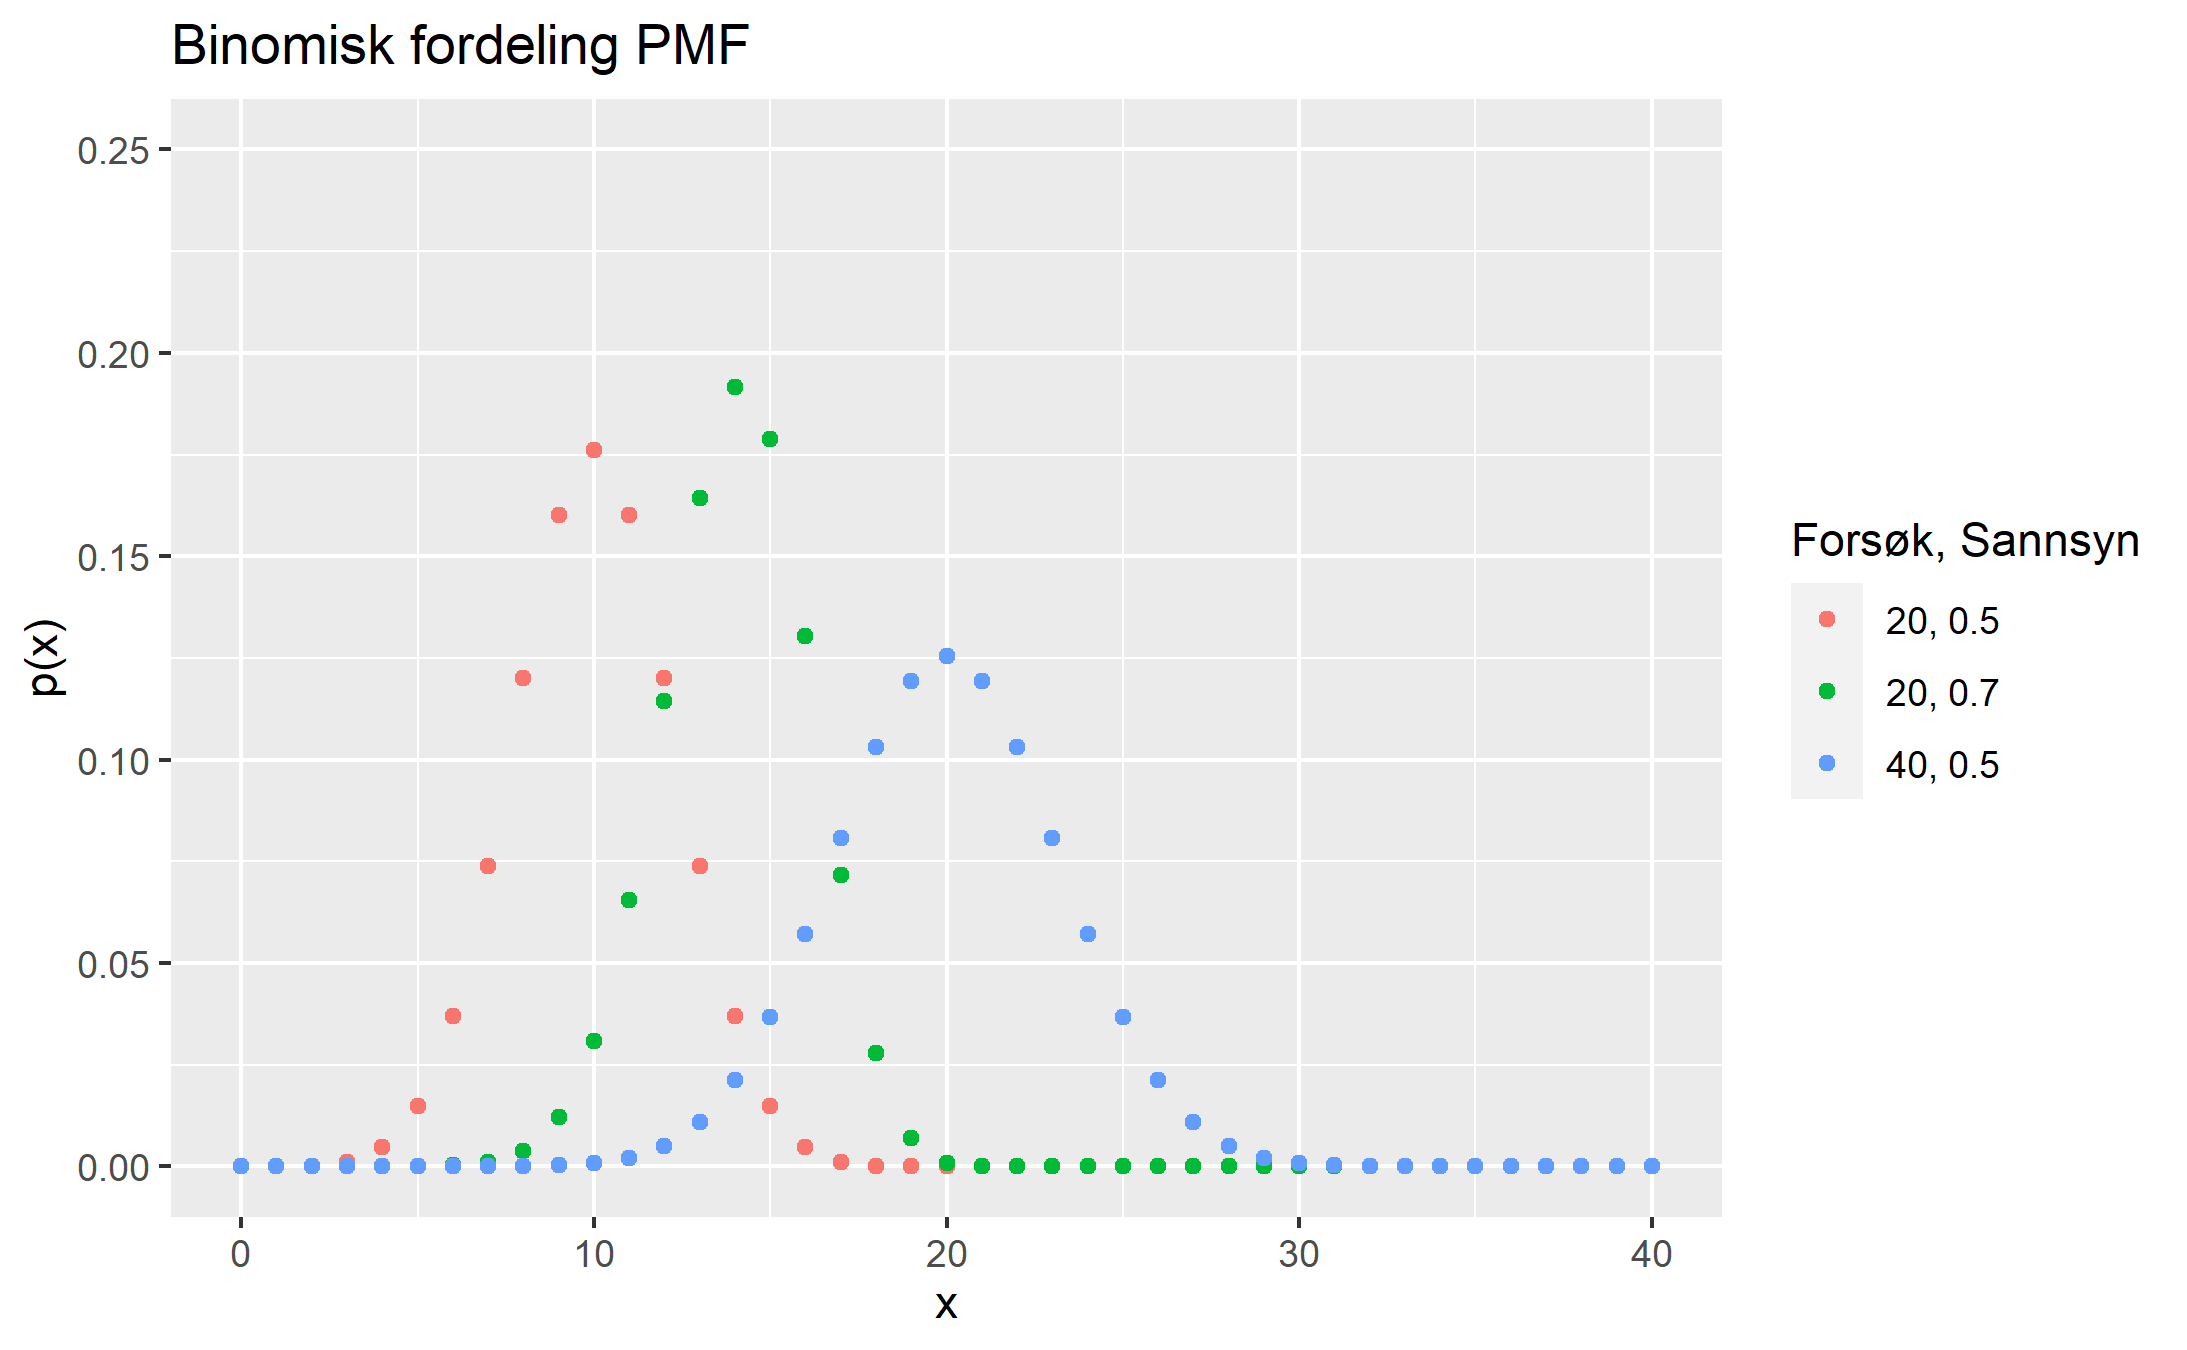
\includegraphics[width=\textwidth]{bilete/binompmf.png}
  \end{minipage}
  \hfill
  \begin{minipage}[b]{0.49\textwidth}
    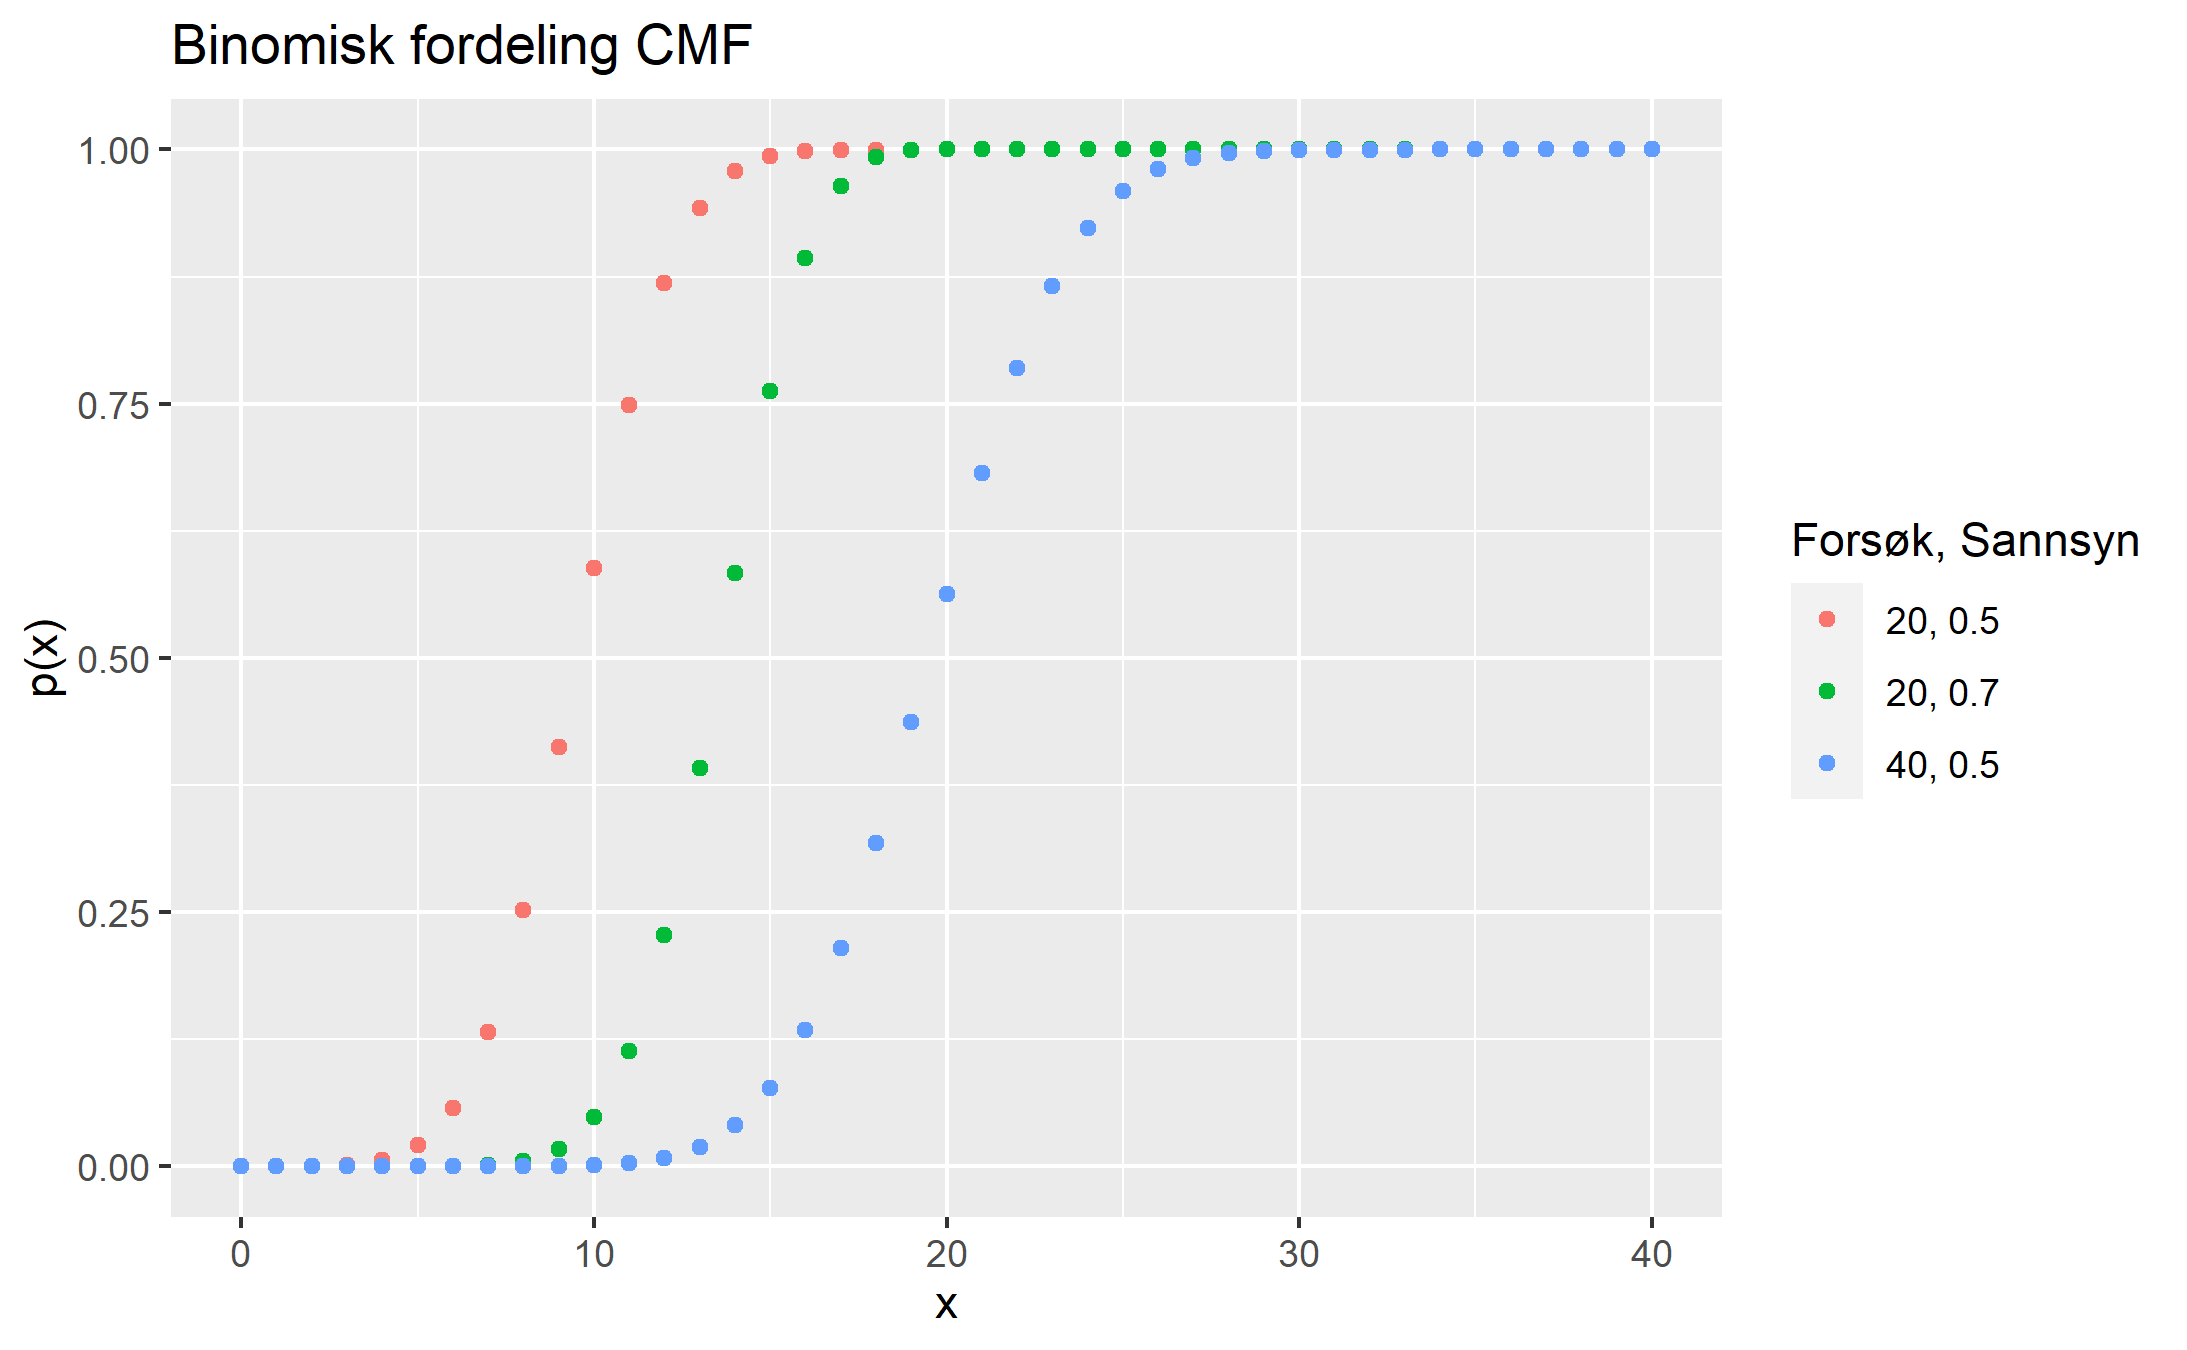
\includegraphics[width=\textwidth]{bilete/binomcdf.png}
  \end{minipage}
\end{figure}

Om $X$ er antalet vellukka hendingar i $n$ bernoulli forsøk er $X$ binomisk fordelt. Den har parameter $p$ for sannsynet for eit vellukka forsøk og $n$ for antal forsøk totalt.

\begin{equation}
    f(x; n, p) = b(x; n, p) = \binom{n}{x}p^x (1-p)^{n-x}
\end{equation}

\begin{equation}
    F(x; n, p) = P(X \leq x) = \sum_{i = 0}^{x} \binom{n}{i}p^i(1-p)^{n-i}
\end{equation}

\begin{equation}
    E[X] = np, \qquad \text{Var}(X) = np(1-p)
\end{equation}

\subsubsection{Bernoulli Prosessen} \label{chap:bernoulli}
For å forstå binomisk fordeling og når denne fordelinga er aktuelle må ein forstå bernoulli prosessen. Under ein streng definisjon, er ein bernoulli prosess ein prosess med følgande eigenskapar:

\begin{enumerate}
    \item Eksperimentet må bestå av gjentatte forsøk.
    \item Kvart forsøk har utfall som er enten vellukka eller mislukka.
    \item Sannsynlegheita for eit vellukka eksperiment $p$ må vere konstant.
    \item Forsøka må vere uavhengige.
\end{enumerate}

\subsection{Negativ-binomisk fordeling}
\begin{figure}[H]
  \centering
  \begin{minipage}[b]{0.49\textwidth}
    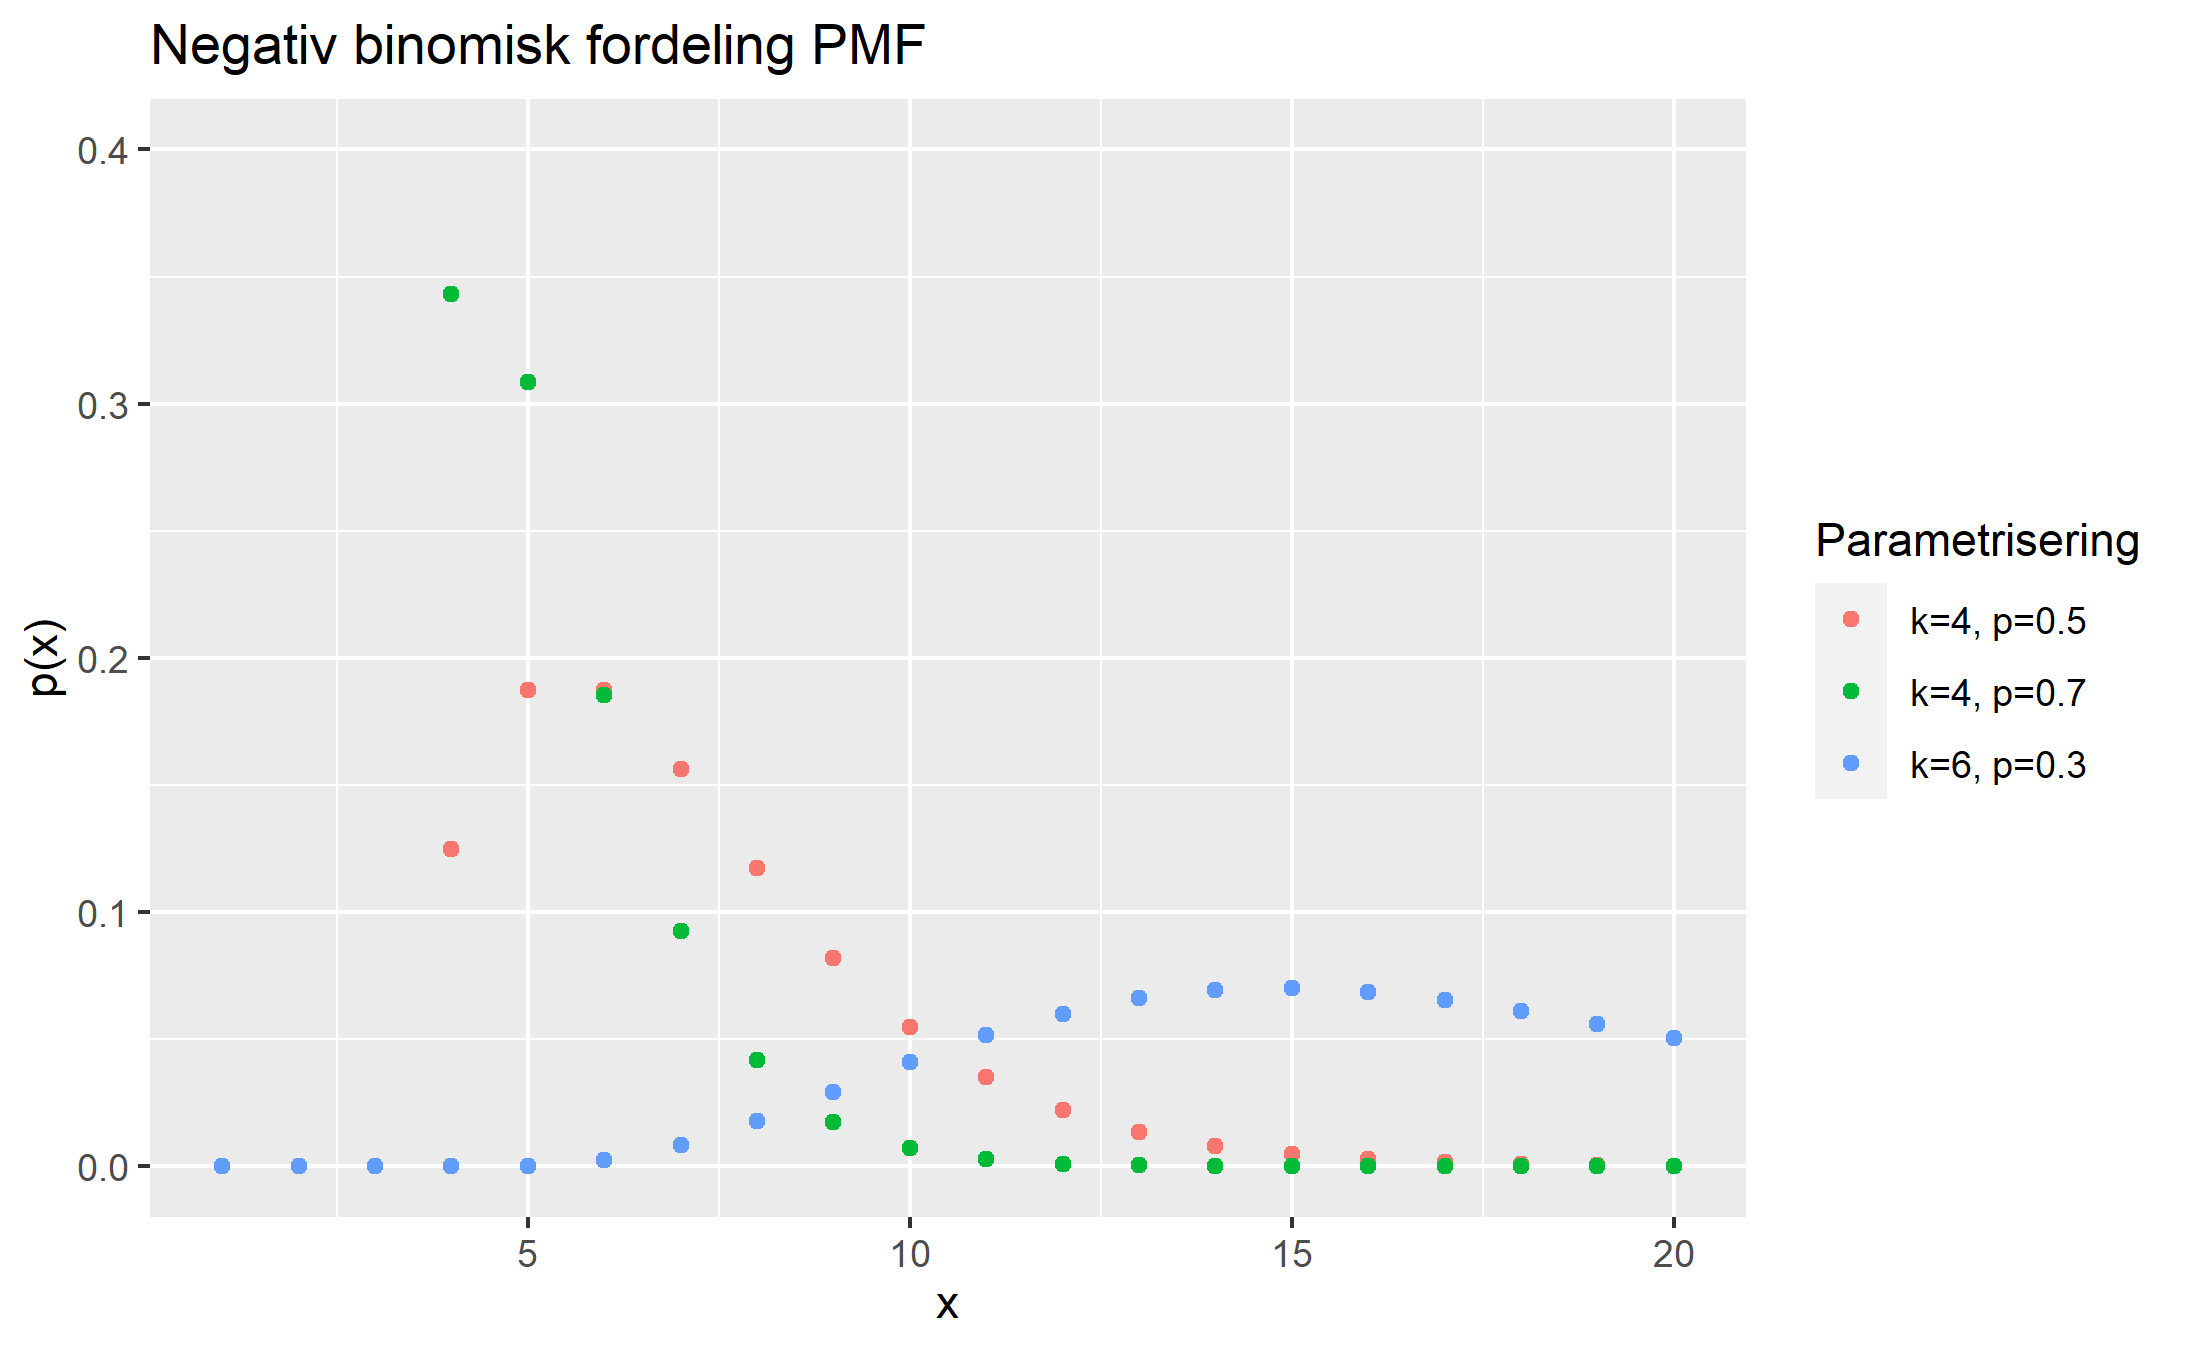
\includegraphics[width=\textwidth]{bilete/negbinpmf.png}
  \end{minipage}
  \hfill
  \begin{minipage}[b]{0.49\textwidth}
    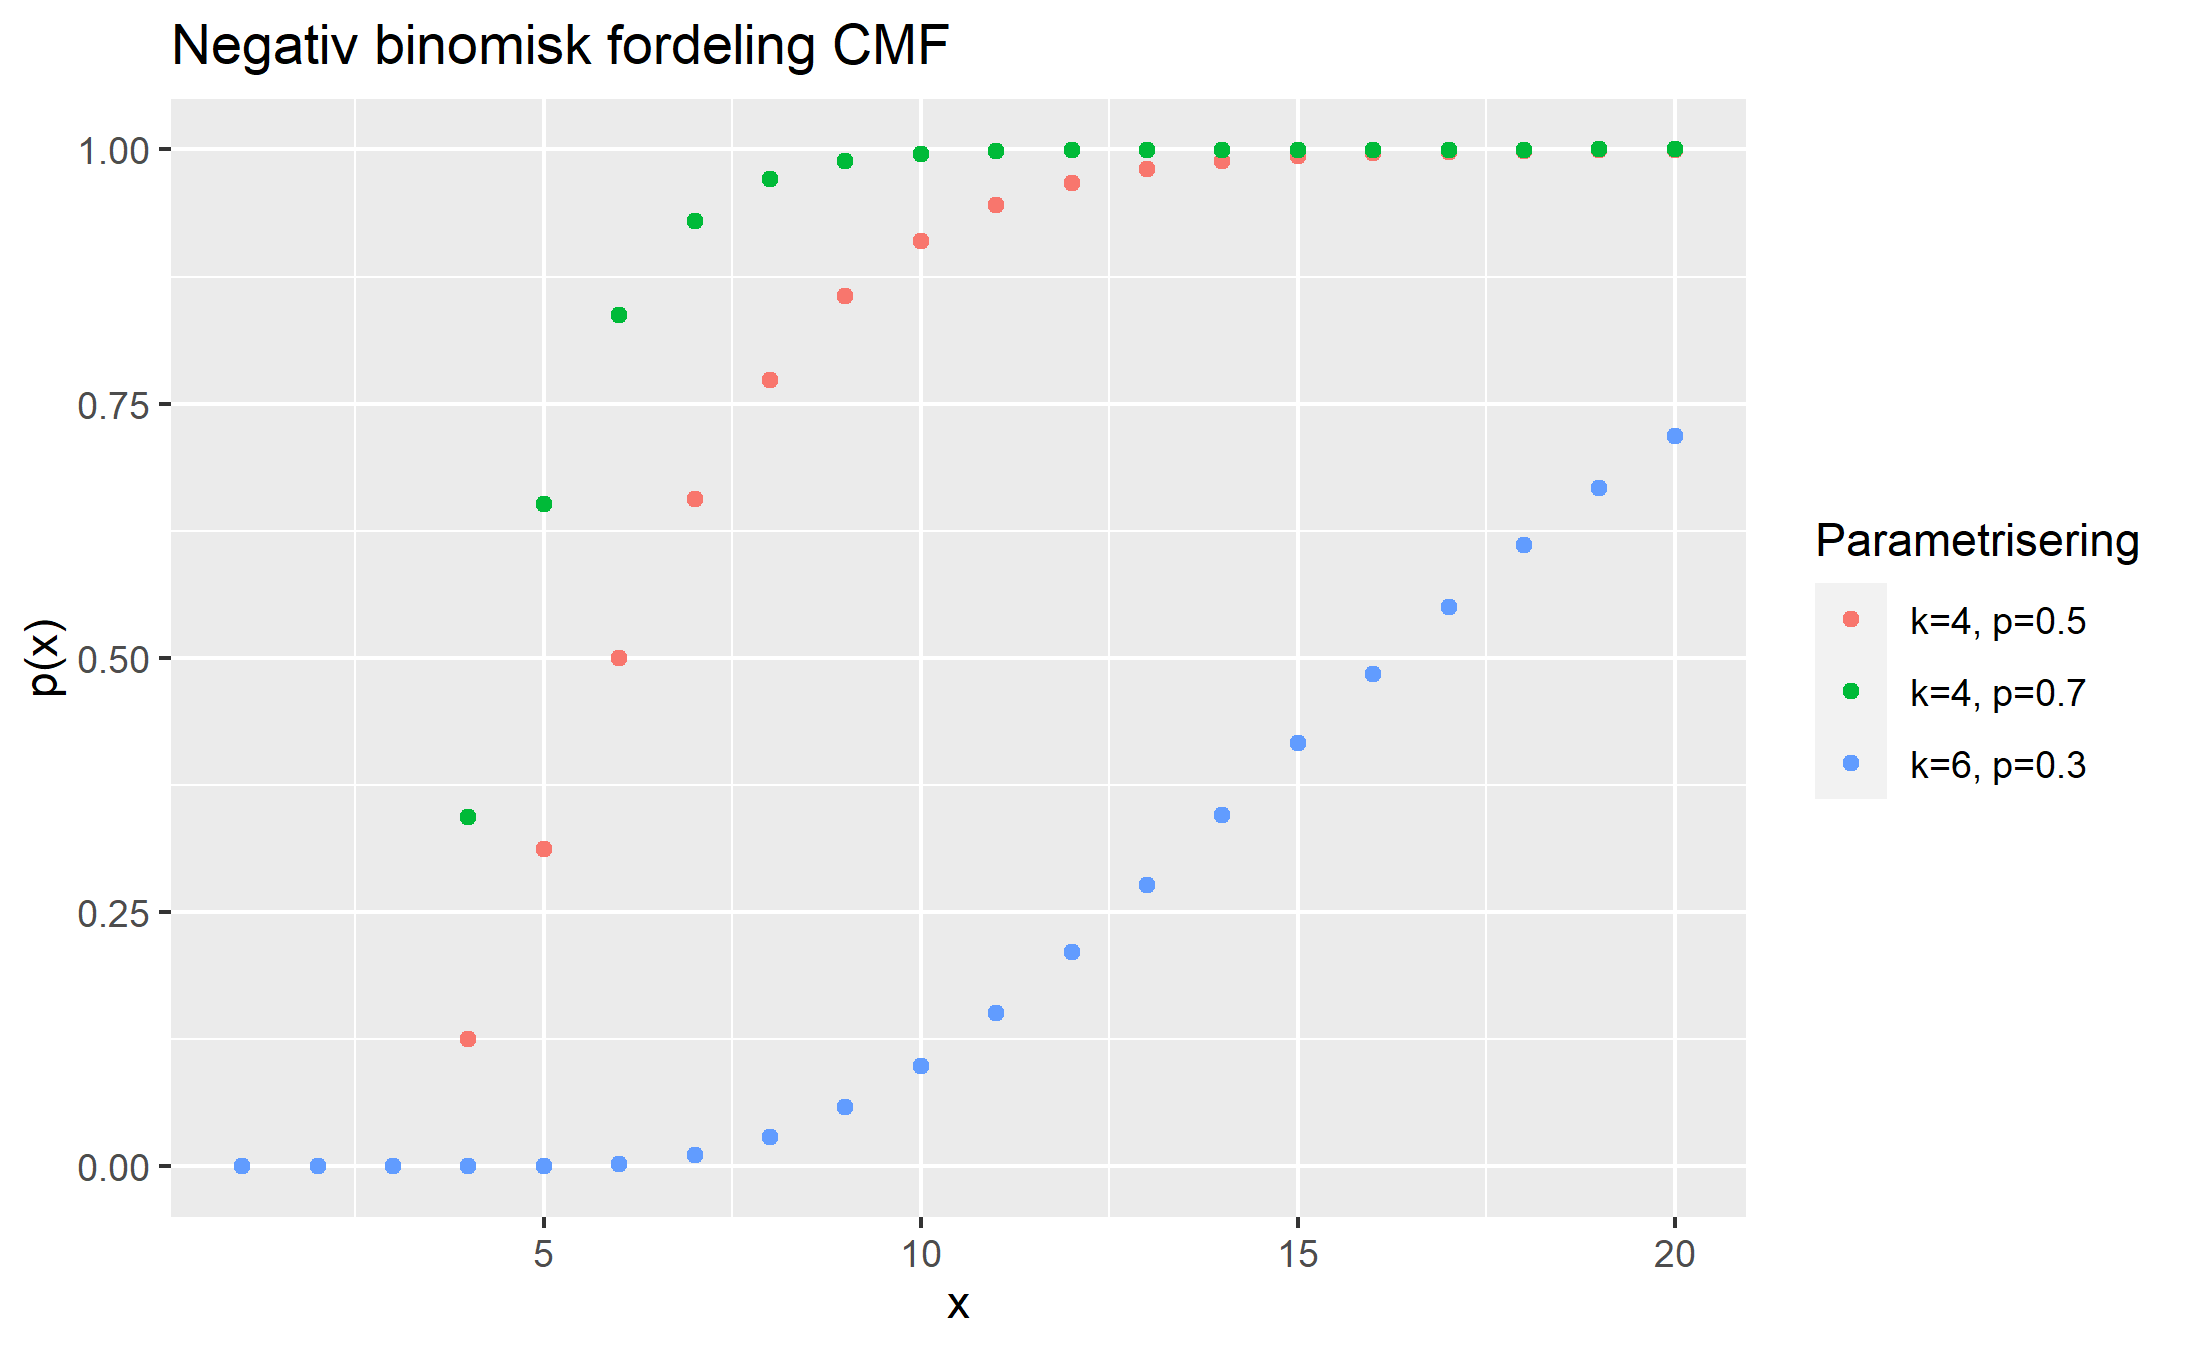
\includegraphics[width=\textwidth]{bilete/negbincdf.png}
  \end{minipage}
\end{figure}
Om eksperimentet følger same eigenskap som bernoulli prosess en \ref{chap:bernoulli}, men istadenfor lar me $X$ = Nummeret på forsøket der suksess $k$ tar stad. Då er $X$ negativ binomisk fordelt. 

\begin{equation}
    f(x; k, p) = b^*(x; k, p) = \binom{x - 1}{k - 1}p^k (1-p)^{x - k}
\end{equation}

\begin{equation}
    F(x; k, p) = P(X \leq x) = \sum_{i = 0}^{x} \binom{i - 1}{k - 1}p^k (1-p)^{i - k}
\end{equation}

\begin{equation}
    E[X] = \frac{k}{p}, \qquad \text{Var}(X) = k\frac{1-p}{p^2}
\end{equation}

\subsubsection{Alternative parametriseringar}
Det er viktig å bemerke seg at det er fleire parametriseringar av negativ-binomisk fordeling. \cite{wiki:negativebinom} Det er 3 variantar av desse. $X$ teller...

\begin{enumerate}
    \item $k$ mislukka gitt $r$ vellukka.
    \item $n$ forsøk gitt $k$ vellukka. (Dette er parametriseringa over)
    \item $r$ vellukka gitt $n$ forsøk. (Dette er binomisk fordeling \ref{chap:binomford})
\end{enumerate}

Dei alternative parametriseringane blir ikkje gått gjennom her, men det er viktigt å vere obs på at desse finst.

\subsection{Multinomisk fordeling}
Ein multinomisk fordeling er ein fleirvariabels parameter og er derfor ikkje plotta som dei andre fordelingane.

\begin{equation}
    f(x:1, \dots, x_k; p_1, \dots, p_k, n) = \frac{n!}{x_1! \dots x_k!}p_1^{x_1}\dots p_k^{x_k}
\end{equation}

\begin{equation}
    E[X_i] = np_i, \qquad \text{Var}(X_i) = np_i(1-p_i), \qquad \text{Cov}(X_i, X_j) = -np_ip_j
\end{equation}

\subsubsection{Multinomisk eksperiment}
Eit binomisk eksperiment (sjå \ref{chap:bernoulli}) blir eit multinomisk eksperiment om me lar forsøka he fleire utfall. Dei andre eigenskapane er dei same.

\subsection{Geometrisk fordeling}
\begin{figure}[H]
  \centering
  \begin{minipage}[b]{0.49\textwidth}
    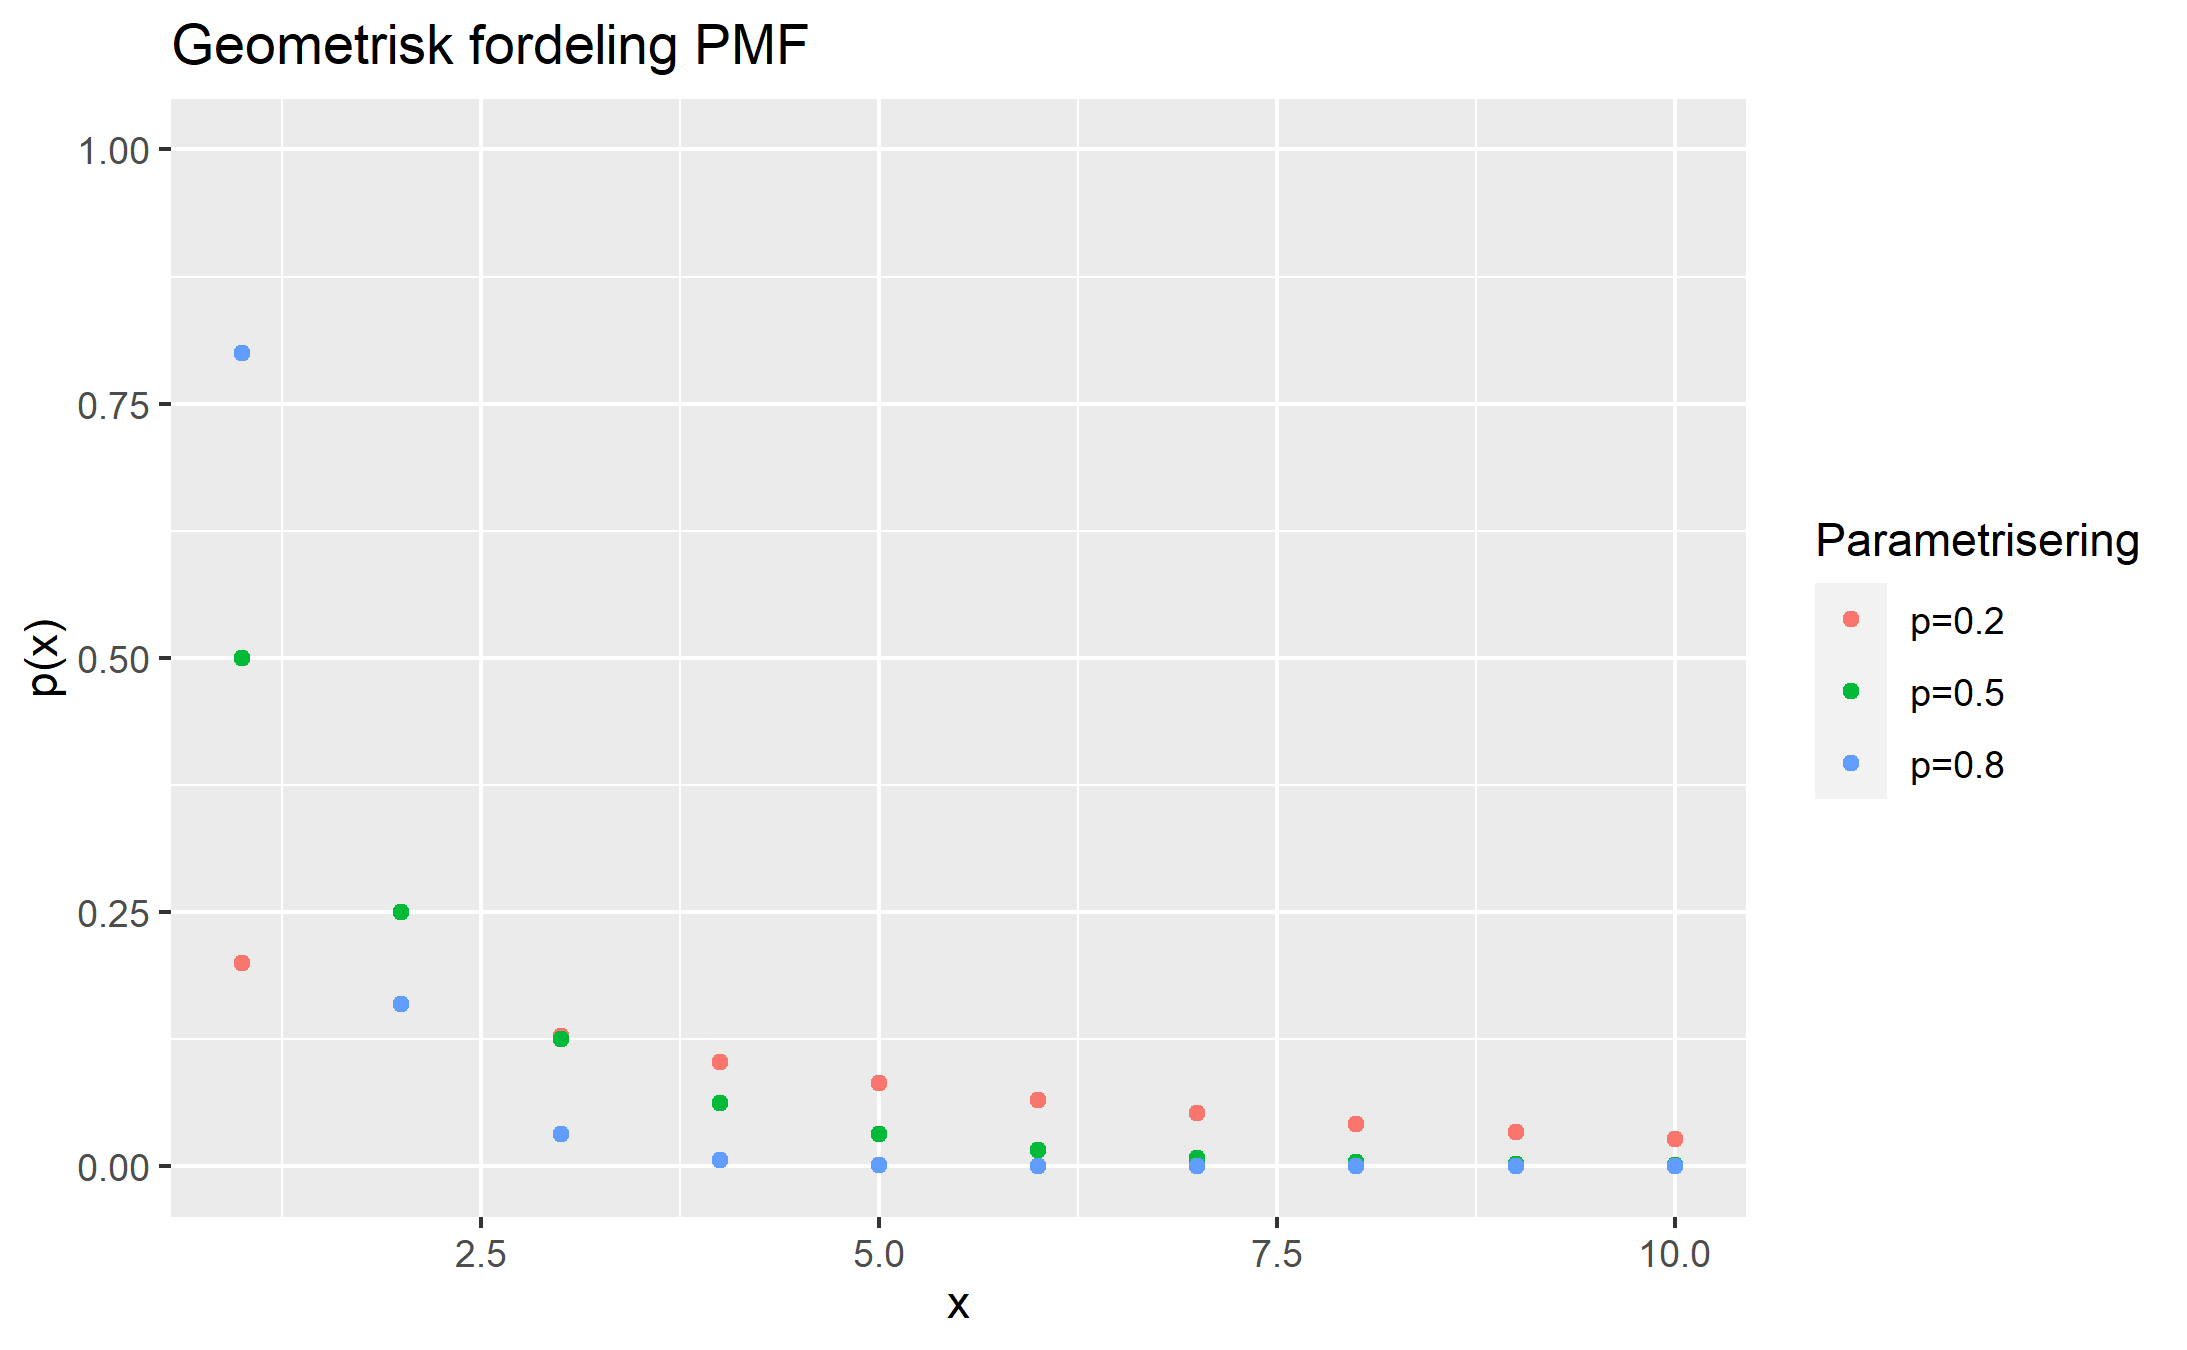
\includegraphics[width=\textwidth]{bilete/geompmf.png}
  \end{minipage}
  \hfill
  \begin{minipage}[b]{0.49\textwidth}
    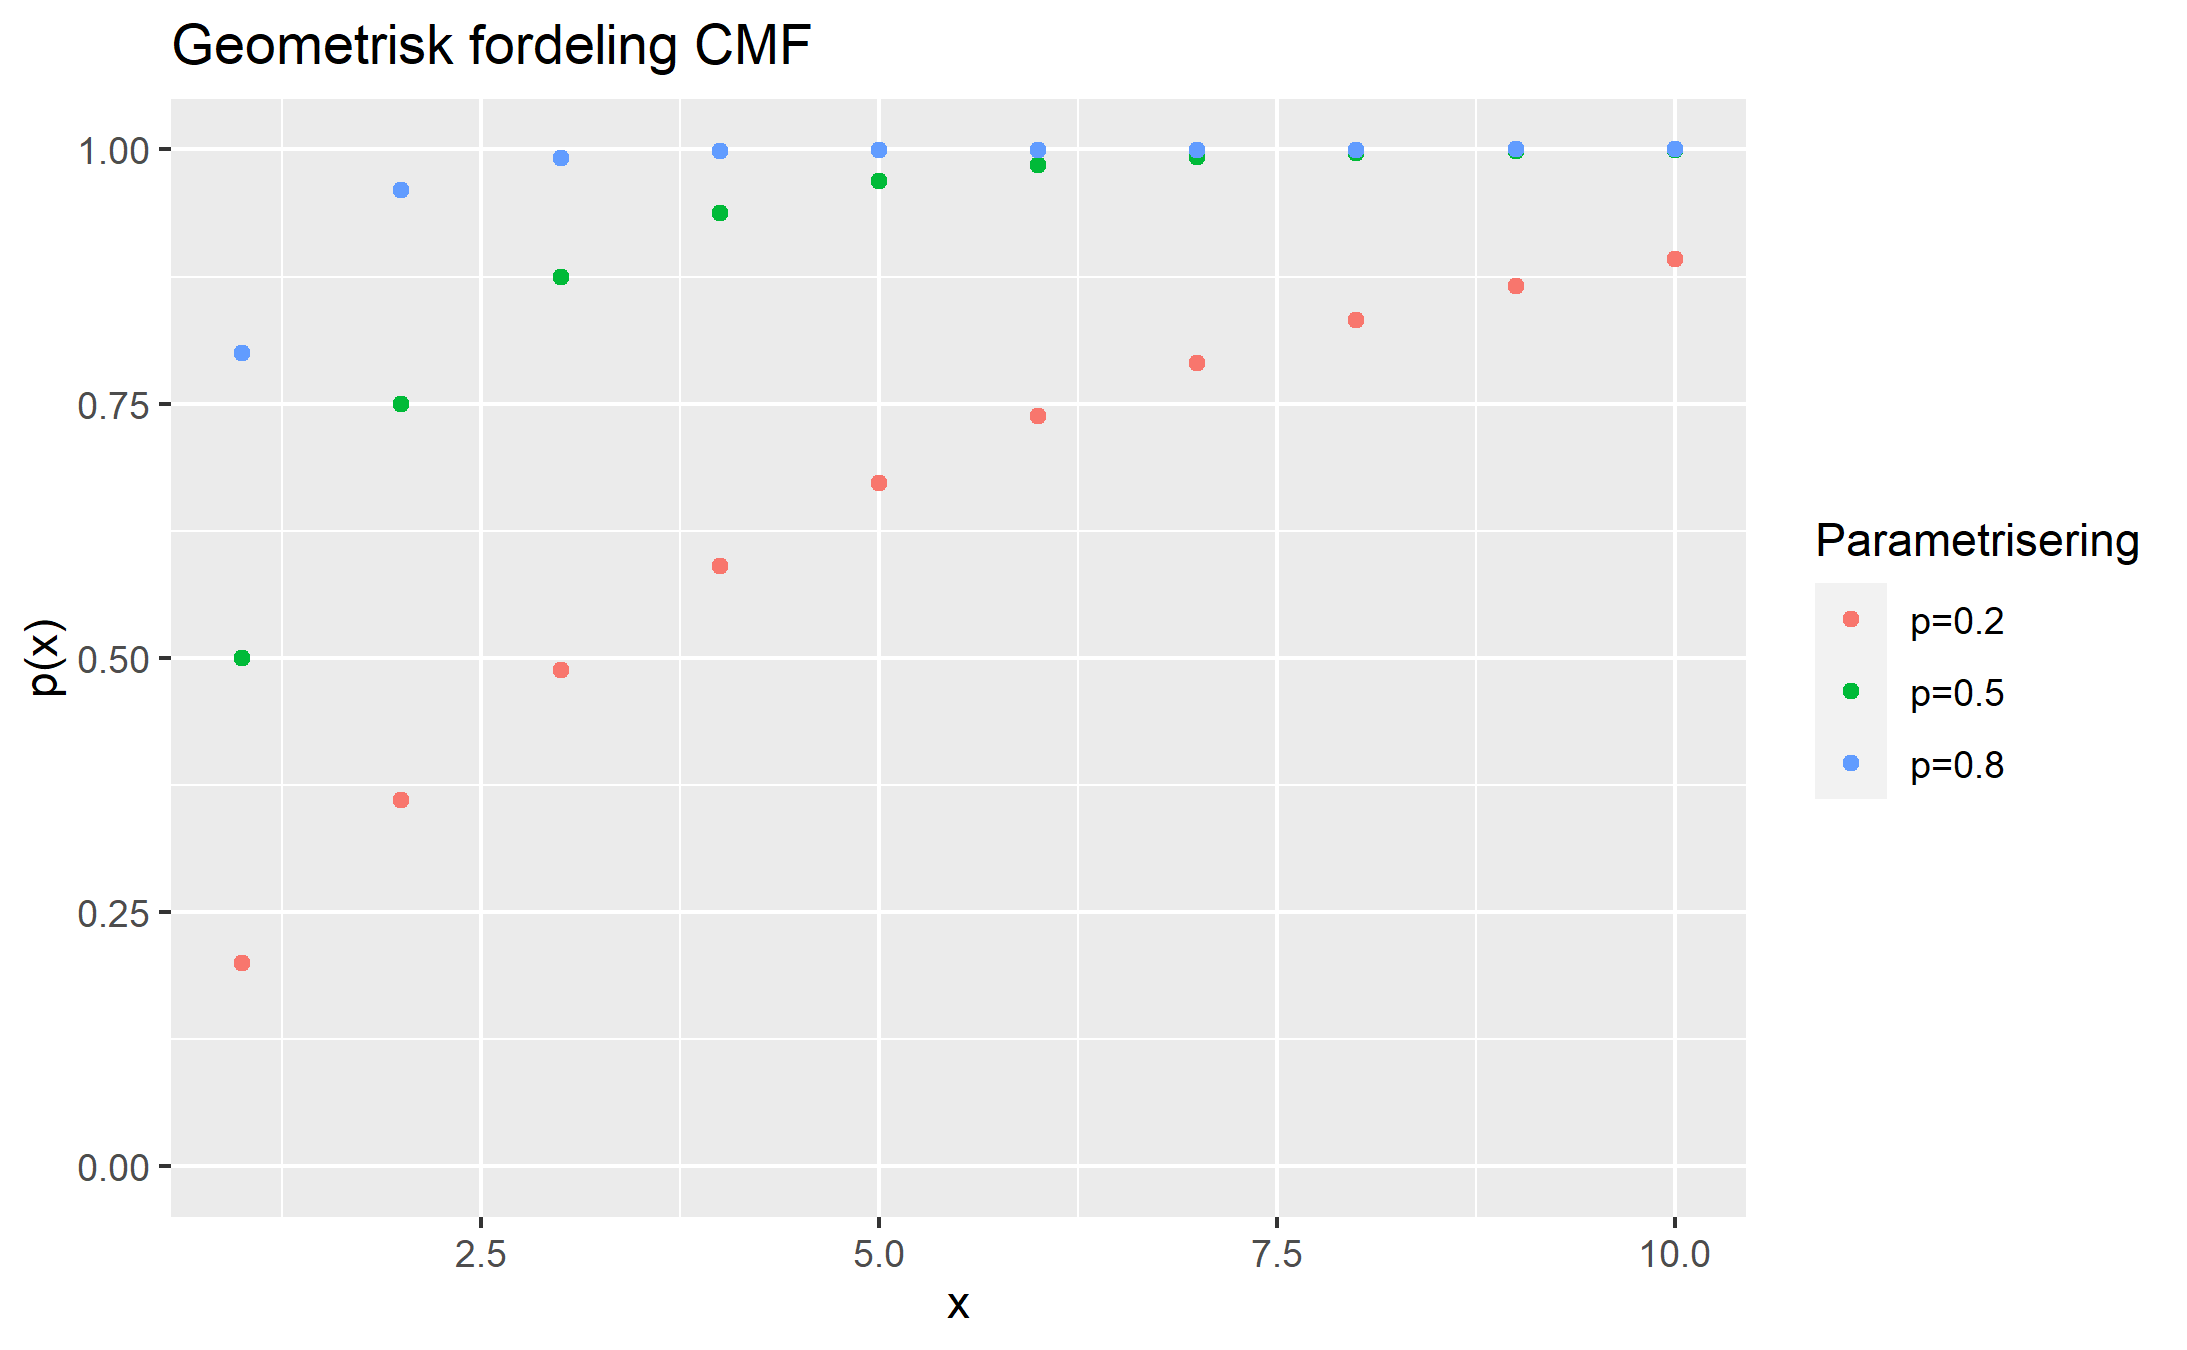
\includegraphics[width=\textwidth]{bilete/geomcdf.png}
  \end{minipage}
\end{figure}

Eit spesialtilfelle av negativ-binomisk fordeling er geometrisk fordeling. Gitt at vi har ein bernoulli prosess \ref{chap:bernoulli}, om $X =$ Antal forsøk inntil 1 suksess, så er $X$ geometrisk fordelt.

\begin{equation}
    f(x; \lambda t) = g(x; 1, p) = (1-p)^{x-1}p, \qquad x = 0, 1, 2, \dots
\end{equation}

\begin{equation}
    F(x; 1, p) = P(X \leq x) = 1 - (1 - p)^x
\end{equation}

\begin{equation}
    E[X] = \frac{1}{p}, \qquad \text{Var}(X) = \frac{1-p}{p^2}
\end{equation}

\subsection{Poissonfordeling}
\begin{figure}[H]
  \centering
  \begin{minipage}[b]{0.49\textwidth}
    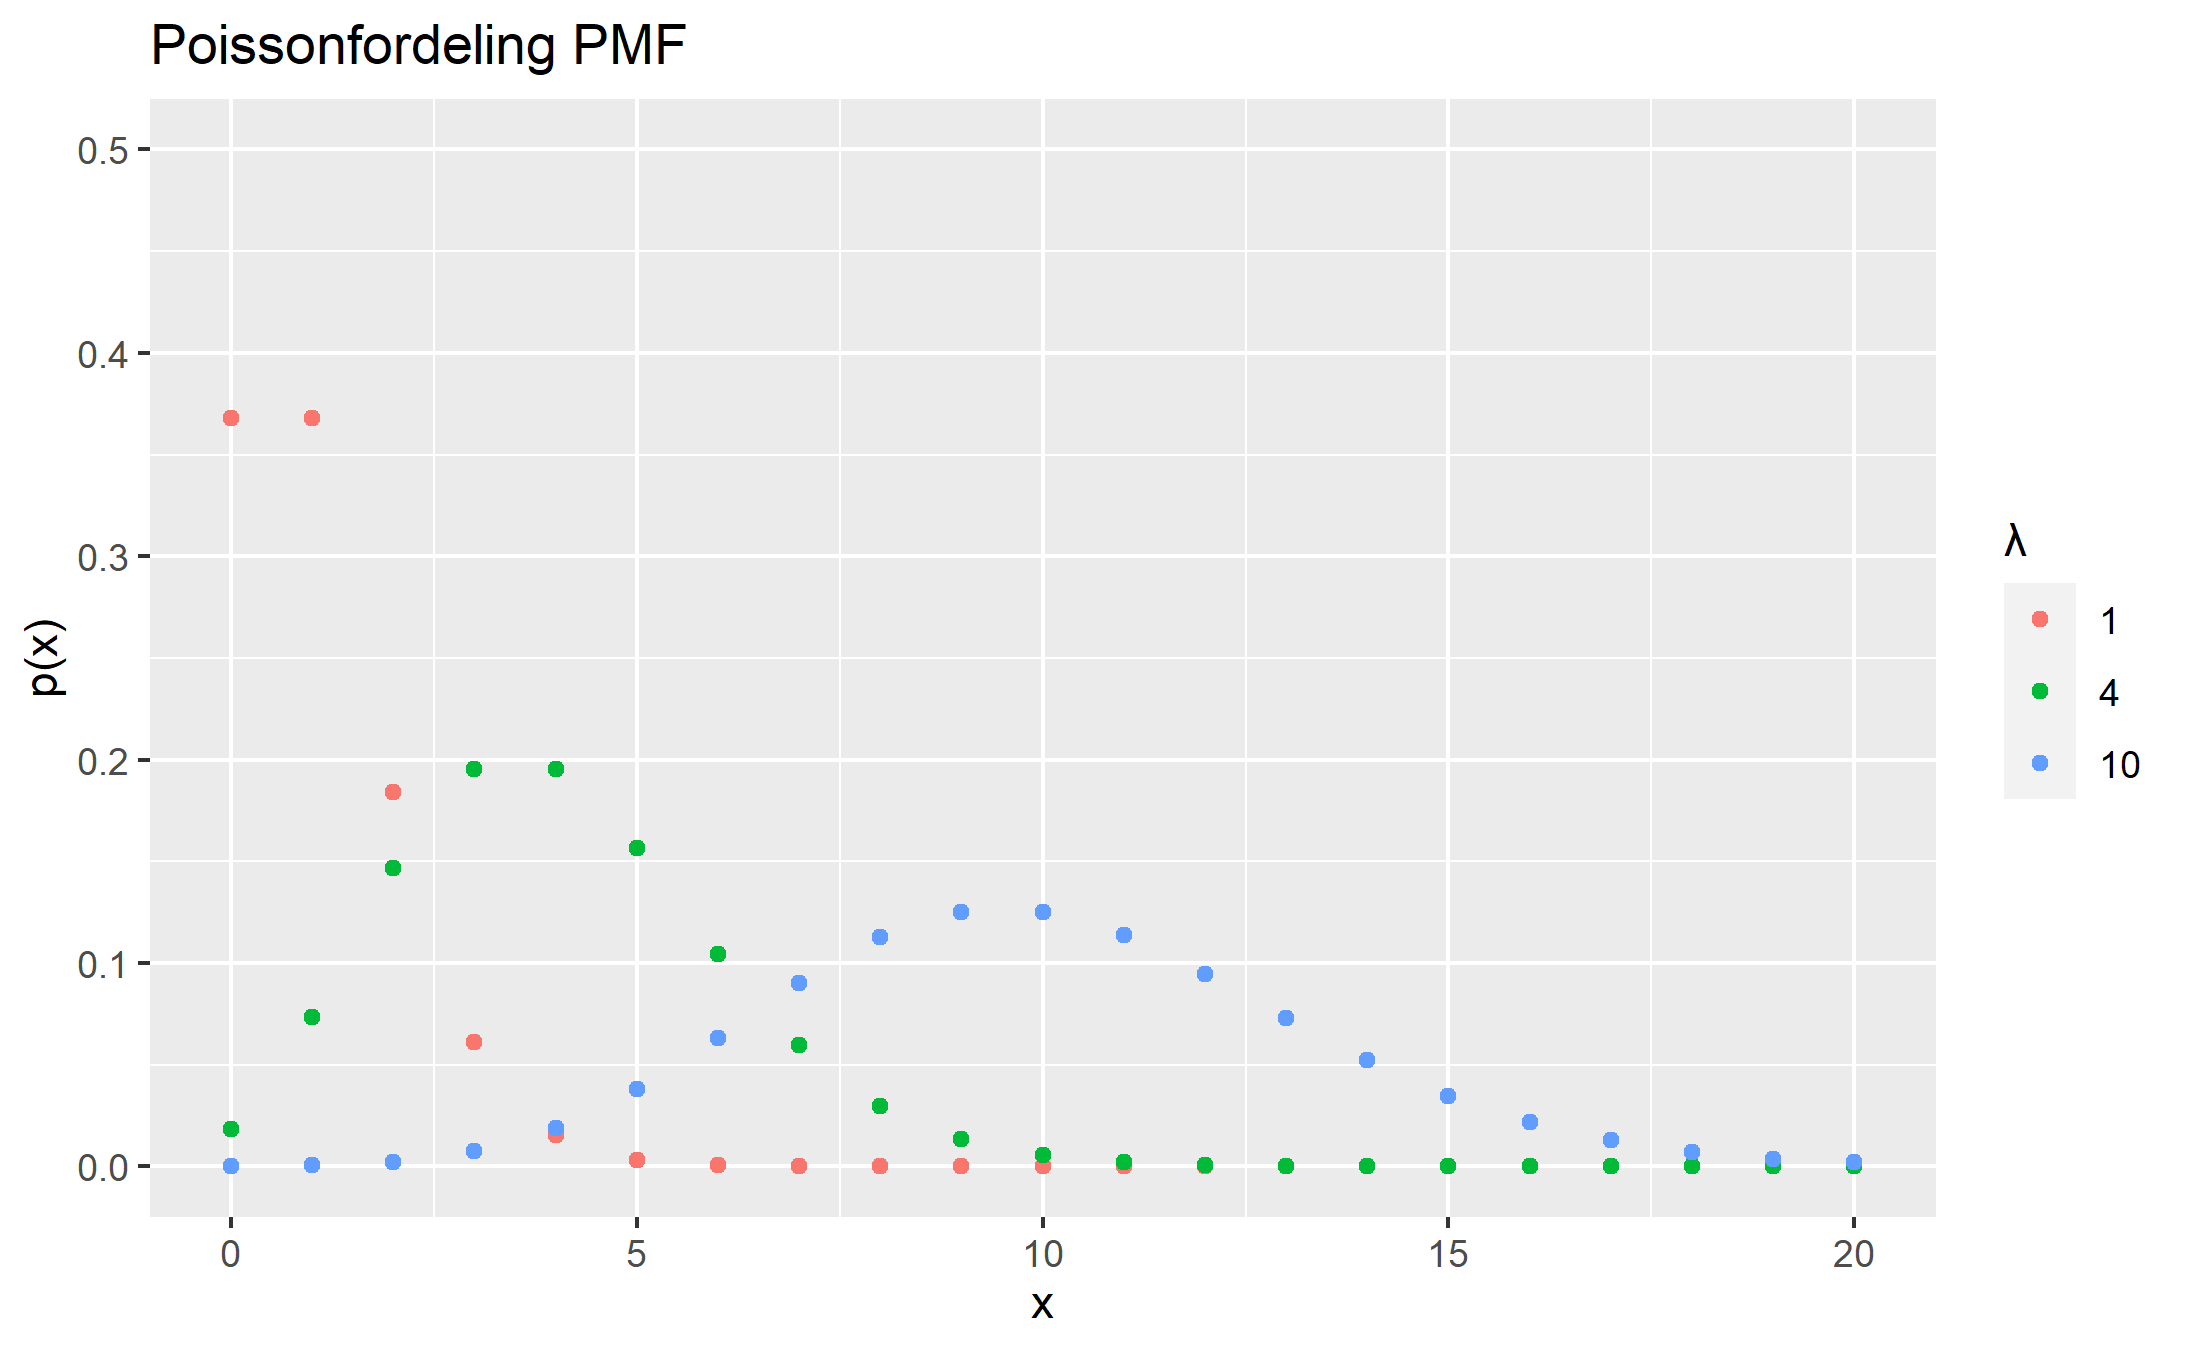
\includegraphics[width=\textwidth]{bilete/poispmf.png}
  \end{minipage}
  \hfill
  \begin{minipage}[b]{0.49\textwidth}
    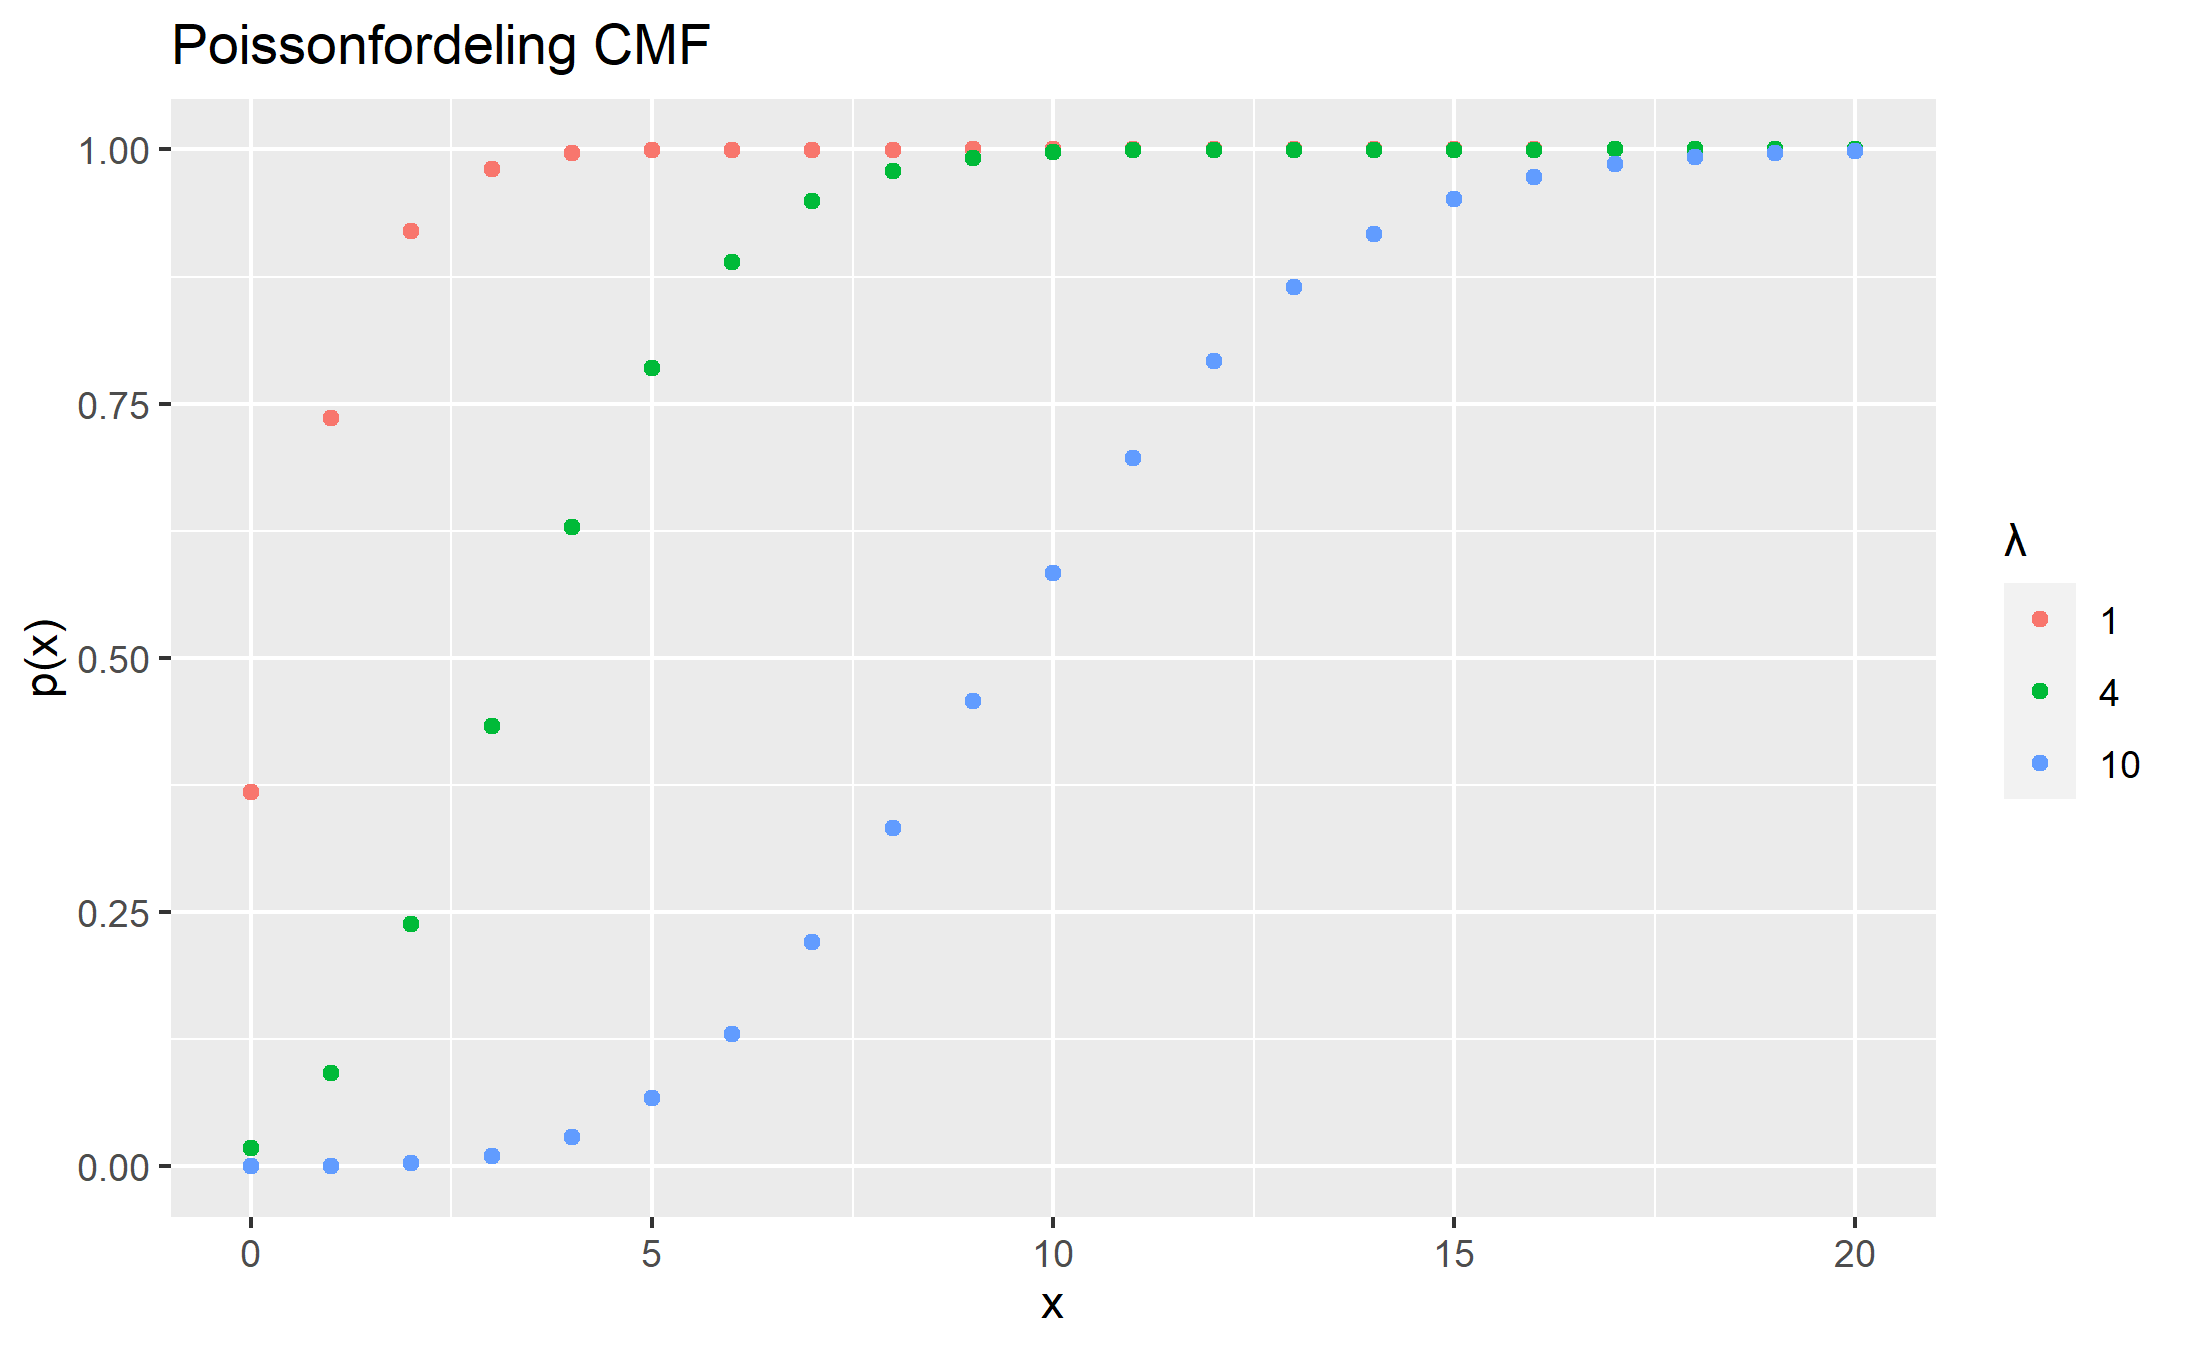
\includegraphics[width=\textwidth]{bilete/poiscdf.png}
  \end{minipage}
\end{figure}

Poissonfordelinga beskriver sannsynet for antalet hendingar som skjer i eit avgrensa plass og/eller tidsrom der hendingane er uavhengige frå kvarandre (Les her for meir om poisson prosessen: \ref{chap:poissonpro}). 

\begin{equation}
    f(x; \lambda t) = p(x; \lambda t) = \frac{e^{-\lambda t}(\lambda t)^x}{x!}, \qquad x = 0, 1, 2, \dots
\end{equation}

\begin{equation}
    F(x; \lambda t) = P(X \leq x) = \sum_{i = 0}^{x} \frac{e^{-\lambda t}(\lambda t)^i}{i!}
\end{equation}

\begin{equation}
    E[X] = \lambda t, \qquad \text{Var}(X) = \lambda t
\end{equation}

\subsubsection{Poisson prosessen}\label{chap:poissonpro}
Ein stokastisk variabel $X$ er poissonfordelt når $X$ er antalet hendingar i ein poisson prosess. Poisson prosessen har følgande eigenskapar:

\begin{enumerate}
    \item Antalet hendingar i eit tidsintervall eller område er uavhengig antalet hendingar i eit anna, disjunkt tidsintervall eller område. Dette gjer at poisson prosessen er \textit{minnelaus }\ref{memless}.
    \item Sannsynet for eit enkelt utfall i eit lite tidsrom eller område er proporsjonalt med størelsen på intervallet eller området og er uavhengig antalet hendingar utanfor dette tidsrommet eller området.
    \item Sannsynet for at meir enn ein hending vil skje i eit tidsintervall er neglisjerbart.
\end{enumerate}

\subsection{Hypergeometrisk fordeling}
\begin{figure}[H]
  \centering
  \begin{minipage}[b]{0.49\textwidth}
    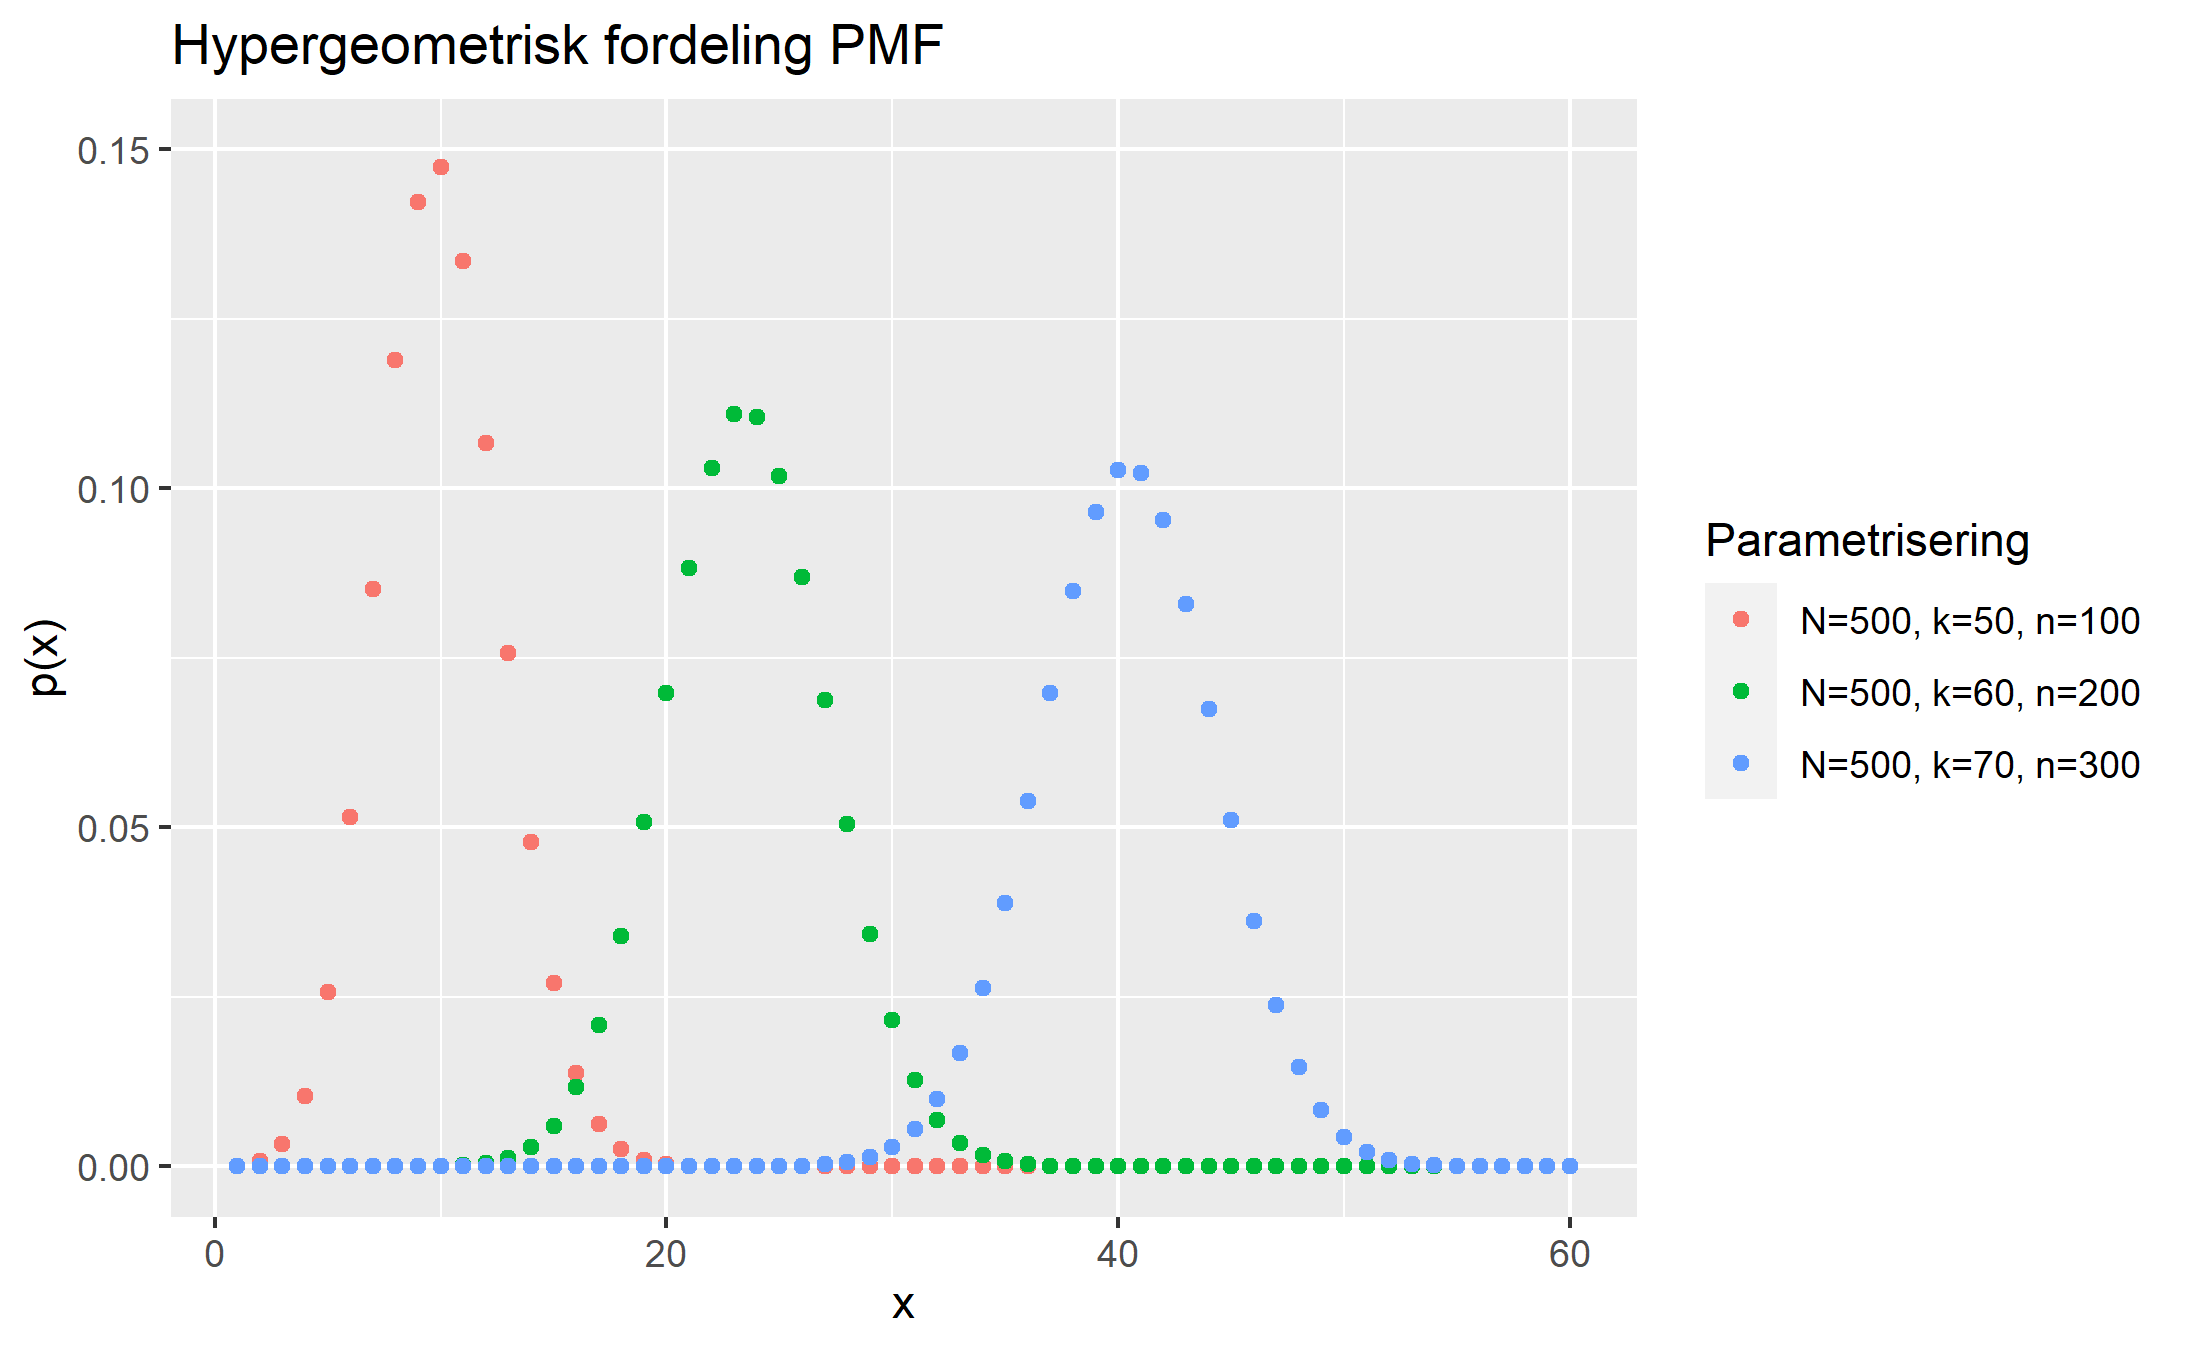
\includegraphics[width=\textwidth]{bilete/hypergeompmf.png}
  \end{minipage}
  \hfill
  \begin{minipage}[b]{0.49\textwidth}
    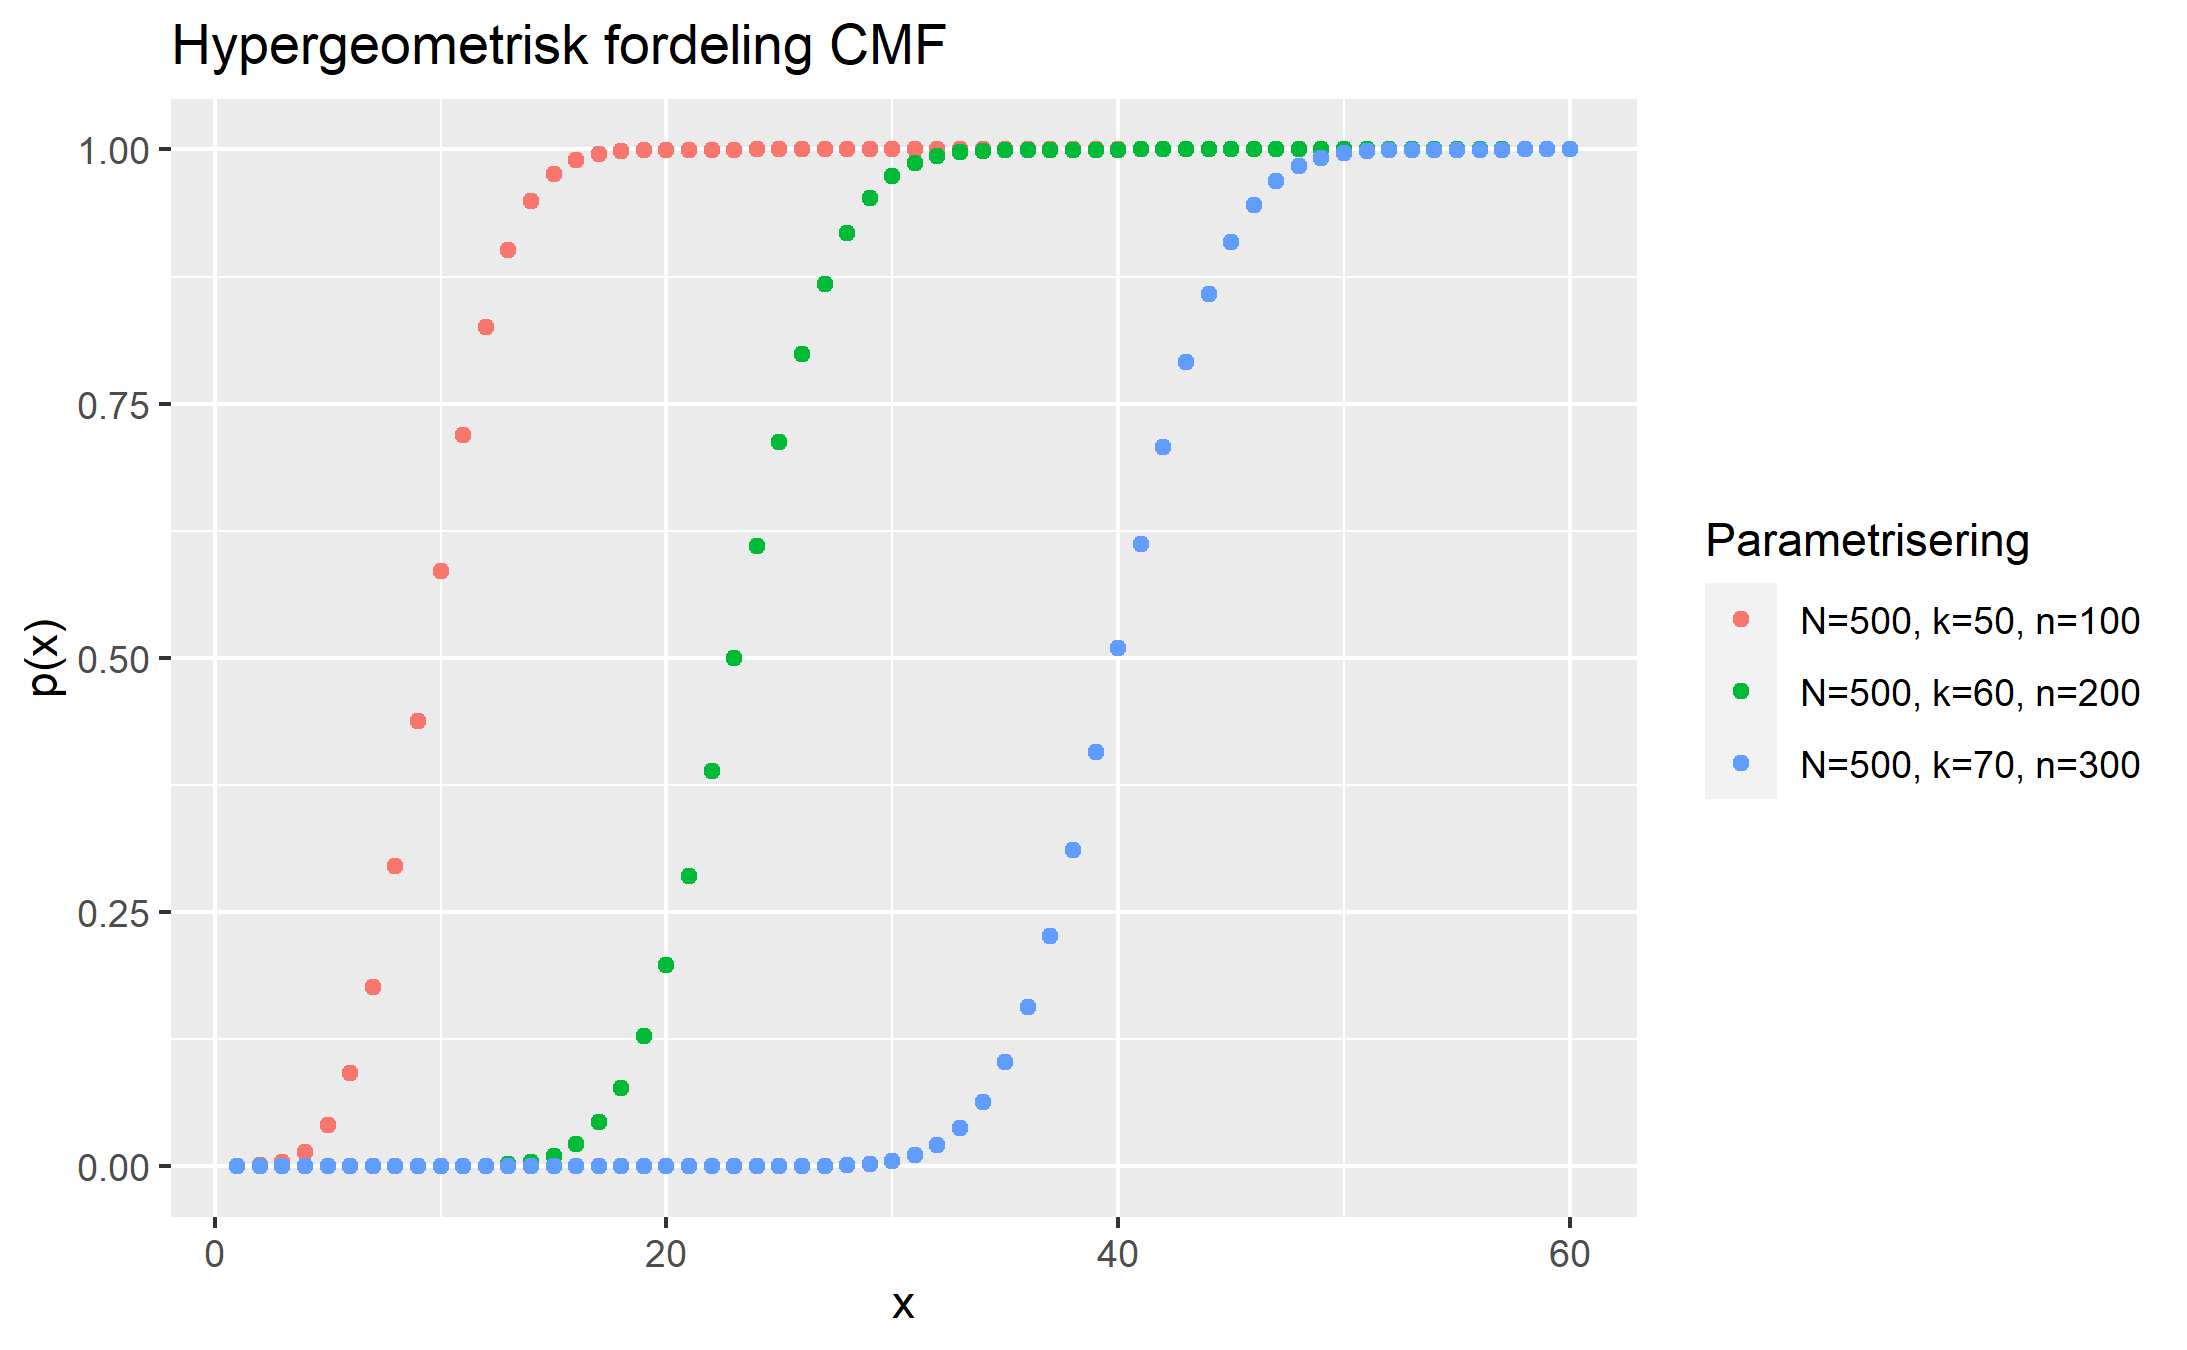
\includegraphics[width=\textwidth]{bilete/hypergeomcmf.png}
  \end{minipage}
\end{figure}

Når $X$ er antal vellukka forsøk i eit hypergeometrisk eksperiment (sjå: \ref{chap:hypergeom}) så er den stokastiske variabelen $X$ hypergeometrisk fordelt. Me har parametra $N$ for populasjonsstørelsen, $n$ for antal forsøk og $k$ for antal vellukka/ønska element i populasjonen.

\begin{equation}
    f(x; N, n, k) = h(x; N, n, k) = \frac{\binom{k}{x}\binom{N-k}{n-k}}{\binom{N}{n}},
    \qquad \max\{0, n - (N - k)\} \leq x \leq \min \{n, k\}
\end{equation}

\begin{equation}
    F(x; N, n, k) = P(X \leq x) = \sum_{i = 0}^{x} \frac{\binom{k}{i}\binom{N-k}{n-k}}{\binom{N}{n}}
\end{equation}

\begin{equation}
    E[X] = n\frac{nk}{N}, \qquad \text{Var}(X) = \frac{N-n}{N-1}\cdot n \cdot \frac{k}{N}\left( 1 - \frac{k}{N}\right)
\end{equation}

\subsubsection{Hypergeometrisk eksperiment}\label{chap:hypergeom}
For å ha eit hypergeometrisk eksperiment må eksperimentet ha følgande eigenskapar

\begin{enumerate}
    \item Eit tilfeldig utvalg på størrelse $n$ er valg uten tilbakelegging frå $N$ moglege.
    \item Av $N$ moglege valg er $k$ rekna som vellukka og $N - k$ rekna som mislukka.
\end{enumerate}

Eit hypergeometrisk eksperiment kan derfor minne om eit binomisk, men eit hypergeometrisk eksperiment har eit sannsyn for eit vellukka forsøk $p$ som ikkje er konstant.

\subsection{Diskret uniform fordeling}
\begin{figure}[H]
  \centering
  \begin{minipage}[b]{0.49\textwidth}
    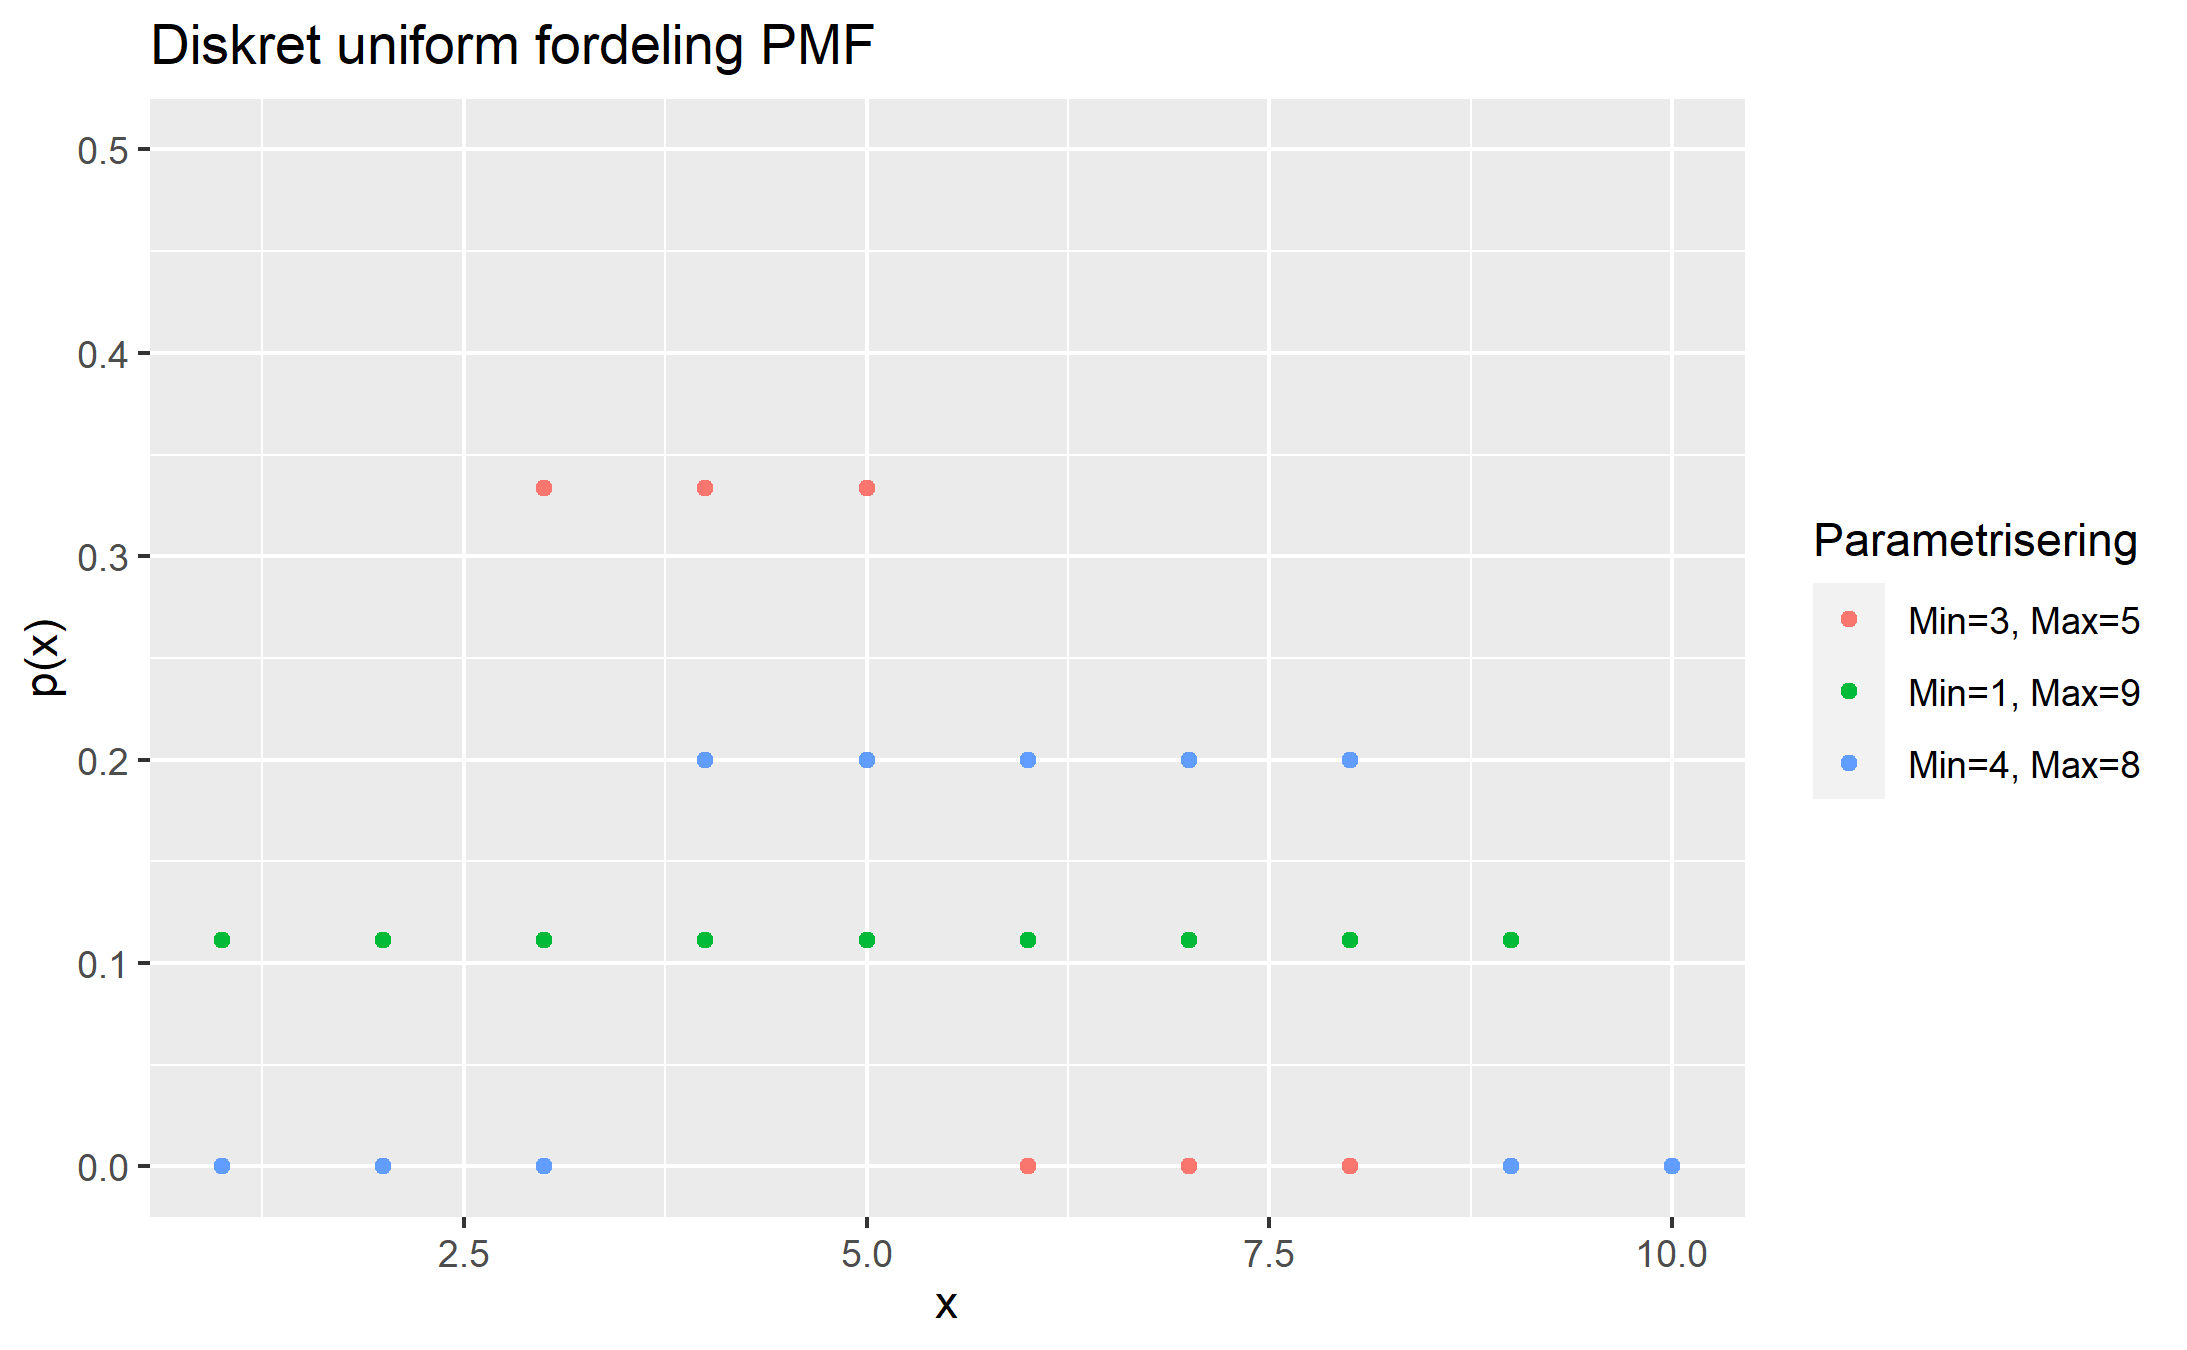
\includegraphics[width=\textwidth]{bilete/diskretuniformpmf.png}
  \end{minipage}
  \hfill
  \begin{minipage}[b]{0.49\textwidth}
    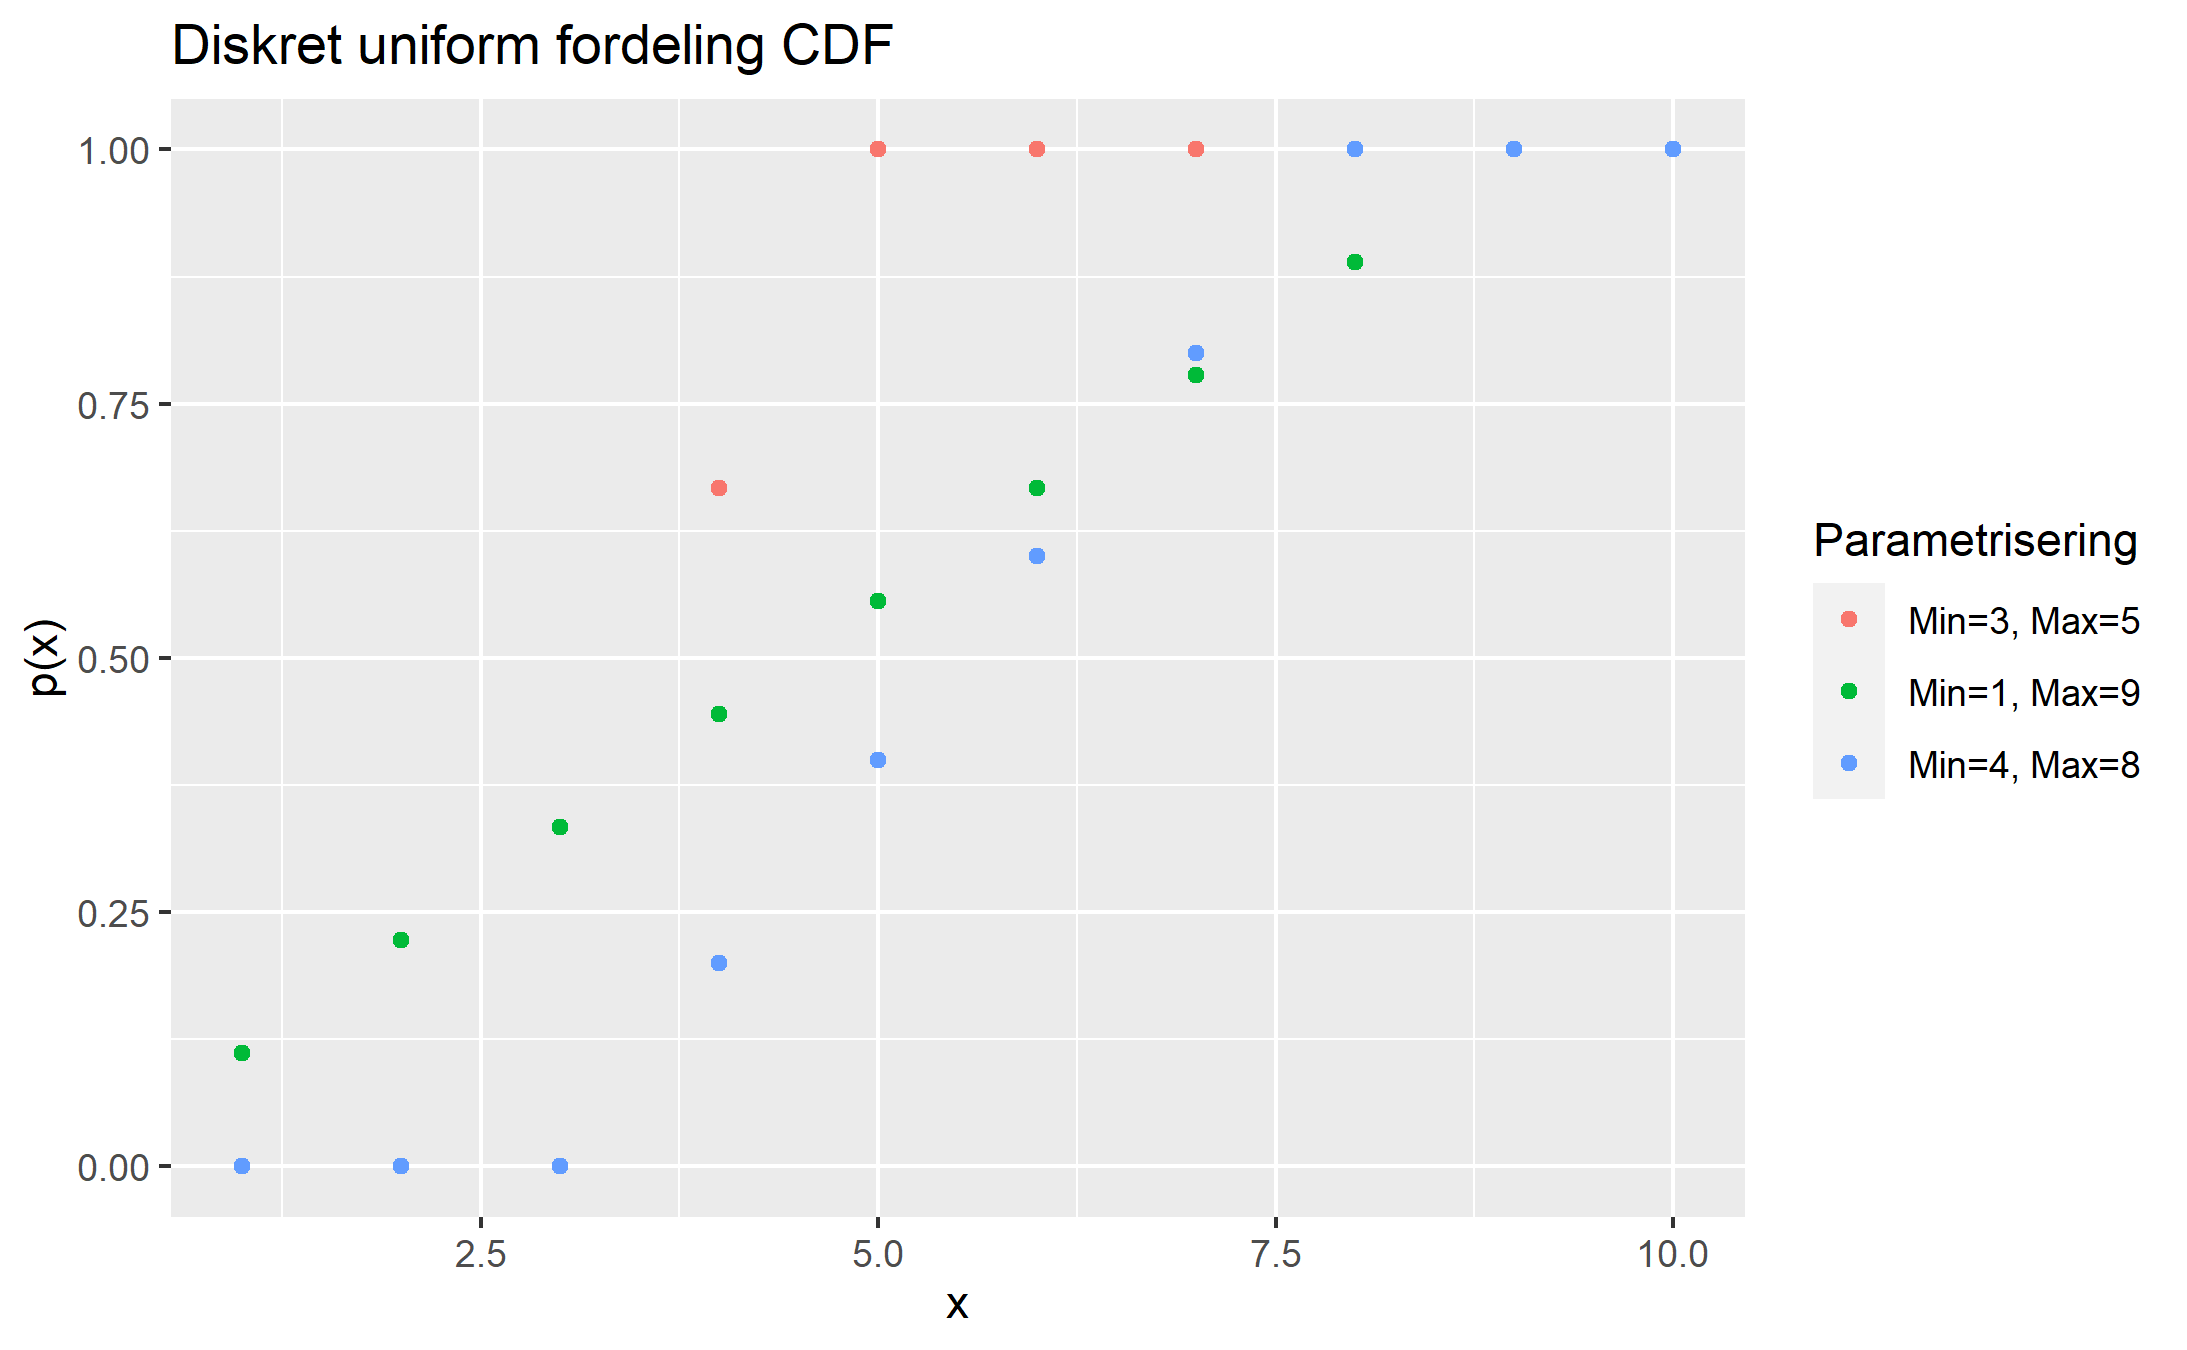
\includegraphics[width=\textwidth]{bilete/diskretuniformcdf.png}
  \end{minipage}
\end{figure}

Den diskrete uniforme fordelinga er ein fordeling der alle moglege utfall er like sannsynleg.

\begin{equation}
    f(x; a, b) = \frac{1}{n}, \qquad x \in \{a, a+1, \dots, b-1, b\}, \qquad n = b - a + 1, \qquad a \leq b
\end{equation}

\begin{equation}
    F(x; a, b) = P(X \leq x) = \frac{\lfloor x \rfloor - a + 1}{n}
\end{equation}

\begin{equation}
    E[X] = \frac{a + b}{2}, \qquad \text{Var}(X) = \frac{(b - a + 1)^2 - 1}{12}
\end{equation}

\section{Kontinuerlege sannsynlegheitsfordelingar}

\subsection{Eksponensialfordeling}\label{eksp}

\subsubsection{Skalaparametrisering}
\begin{equation}
    f(x) = \frac{1}{\beta} e^{-\frac{x}{\beta}},  \quad  x \geq 0
\end{equation}

\begin{equation}
    F(x) = \int_{0}^x f(t) dt = 1 - e^{-\frac{x}{\beta}}
\end{equation}

\begin{equation}
    E[X] = \int_{-\infty}^{\infty} xf(x) = \frac{1}{\beta}
\end{equation}

\begin{equation}
    Var[X] = E[X^2] - E[X]^2 = \beta^2
\end{equation}

\subsection{Hastigheitsparametrisering}

\begin{equation}
    f(x) = \lambda e^{\lambda x},  \quad  x \geq 0
\end{equation}

\begin{equation}
    F(x) = \int_{0}^x f(t) dt = 1 - e^{- \lambda x}
\end{equation}

\begin{equation}
    E[X] = \int_{-\infty}^{\infty} xf(x) = \frac{1}{\lambda}
\end{equation}

\begin{equation}
    Var[X] = E[X^2] - E[X]^2 = \frac{1}{\lambda^2}
\end{equation}

\subsubsection{Eksponensialfordelingen og minnelausheit} \label{memless}
Eksponensialfordelinga blir ofte kalla for minnelaus. \cite{wiki:memless} Denne eigenskapen kan bli synt slik med følgande eksempel. Sjå føre deg at du har ei lyspære som har lyst i $300$ timar. Kva er sannsynlegheita for at den vil lyse i $500$ timar til? Om me lar $X$ være den stokastiske variabelen $X = \text{Levetid til ei lyspære i antal timar}$ så vil spørsmålet om levetid matematisk kunne formulerast slik (vha Bayes Teorem \cite{wiki:bayes}):

\begin{equation}
    P(X > 500 + 300 | X > 300) = \frac{P(X > 800 \cap X > 300)}{P(x > 300)} = \frac{P(X > 800)}{P(X > 300)} 
\end{equation}

Ved $P(X > x) = 1 - P(X \leq x) = 1 - (1 - e^\frac{-x}{\beta}) = e^\frac{-x}{\beta}$ får vi at

\begin{equation}
    \frac{P(X > 800)}{P(X > 300)} = \frac{e^\frac{-800}{\beta}}{e^\frac{-300}{\beta}} = e^\frac{-500}{\beta} = P(X > 500)
\end{equation}

Dette gir oss formelen

\begin{equation}
    P(X > t + s | X > s) = P(X > t)
\end{equation}

Dette kan tolkast som at systemet ikkje blir betre eller dårlegare over tid, at lyspæra er like god etter 300 timar som den var da den var ny og at sannsynet for at den ryk i framtida er uavhengig av kor lenge den har lyst frå før. Eksponensialfordelinga er den einaste kontinuerlige sannsynlegheitsfordelinga med denne eigenskapen. Den andre er geometrisk fordeling. 

\subsubsection{NB: Vanleg misforståing}
$P(X > 40 | X > 30) = P(X > 10)$ er korrekt bruk av formelen og \textbf{ikkje}
$P(X > 40 | X > 30) = P(X > 40)$. 